%%%%%%%%%%%%%%%%%%%%%%%%%%%%%%%%%%%%%%%%%%%%%%%%%
%------ LaTeX-Template für Abschlussarbeiten, Prof. Thomas Görne, Dezember 2012 --------
%------ Modified by B.Sc. Julius Neudecker, May 2021 ------
%%%%%%%%%%%%%%%%%%%%%%%%%%%%%%%%%%%%%%%%%%%%%%%%%

%---- Header (mit Formateinstellugen) laden, Inputencoding prxfen ------

%%%%%%%%%%%%%%%%%%%%%%%%%%%%%%%%%%%%%%%%%%%%%%%%%
%---- LaTeX-Header fuer Abschlussarbeiten, Prof. Thomas Goerne, Dez. 2012/Aug. 2013 ----
%------ Modified by B.Sc. Julius Neudecker, May 2021 ------
%%%%%%%%%%%%%%%%%%%%%%%%%%%%%%%%%%%%%%%%%%%%%%%%%

\documentclass[12pt,paper=A4,pointlessnumbers,bibtotoc,liststotoc,DIV=11,BCOR=1mm]{scrreprt}
% BCOR ist die Bindekorrektur (verlorener Rand am linken Blattrand)! Wert haengt von der Art der Heftung ab!!
% DIV ist eine Satzspiegeleinstellung von KOMA-Script / sccreprt.

\pagestyle{headings}

\usepackage[T1]{fontenc} % Font Encoding fuer europaeische Schriften mit Umlauten (Unterstuetzung der Worttrennung)
\usepackage{lmodern} % PostScript-Varianten der TeX Computer Modern-Schriften laden
\usepackage[english]{babel} % Spracheinstellungen fuer Englisch und Neudeutsch laden

\usepackage{graphicx} % Grafikeinbindung (fuer .JPG, .JPEG, .PNG und .PDF, falls pdflatex benutzt wird)
\usepackage[table]{xcolor} % ermoeglicht farbige Schrift und farbige Tabellenzeilen
\definecolor{black}{gray}{0} % Umdefinition der Farbe black, falls noetig (0=schwarz, 1=weiss)
\definecolor{dblue}{rgb}{0.1,0.2,0.6} % Dunkelblau, fuer Hyperlinks
\definecolor{lgray}{gray}{0.9} % Hellgrau, fuer Tabellen (0=schwarz, 1=weiss)

\usepackage{booktabs} % fuer schoene Tabellen

\usepackage[round,authoryear]{natbib} % Literaturverweise mit Name/Jahreszahl in runden Klammern
\bibpunct[:\,]{(}{)}{,}{a}{}{,~}  % Feinformatierung der Natbib-Zitierweise

\usepackage[hyphens]{url}
\usepackage[colorlinks=true,linkcolor=black,citecolor=dblue,urlcolor=dblue]{hyperref} 
\usepackage{hyperref}  
% die Pakete url und hyperref ermoeglichen anklickbare URLs im Quellenverzeichnis in definierter Farbe, 
% sie ermoeglichen den Zeilenumbruch bei langen URLs, und sie erzeugen Hyperlinks (Farbe s.o.) 
% zwischen Quellenverweis und Quellenverzeichnis sowie zwischen label und ref im PDF-Dokument

% Fonteinstellungen fuer Bildunterschriften: Unterschrift serifenlos, "Abbildung" fett (bfseries = bold face series)
\setkomafont{captionlabel}{\sffamily\bfseries}
\setkomafont{caption}{\sffamily}

% Ordner für Grafiken
\graphicspath{ {./images/} }

%% ToDo Notes
\newcommand\todo[1]{\textcolor{red}{#1}}

%------------------------------------------------------------------------------------------------------------------
%------ Eigenstaendigkeitserklaerung im gerahmten Kasten (parbox in einer framebox) ------
%------------------------------------------------------------------------------------------------------------------

\newcommand{\eigen}{
\setlength{\fboxsep}{2ex}
\setlength{\fboxrule}{0.8pt} 
% Einstellungen fuer Rahmenabstand und Rahmendicke der Framebox
\begin{center}
	\fbox{
		\parbox{0.8\linewidth}{
			I hereby confirm that this thesis is my own work and that I have not sought or used inadmissible help of third parties to produce this work and that I have clearly referenced all sources used in this thesis. I have fully referenced and used inverted commas for all text directly or indirectly quoted from a source.
		\par\bigskip\bigskip\bigskip\bigskip
		\hspace*{0.8cm}Place and date \hfill \vorname~\nachname\hspace*{0.8cm}
		}
	}
\end{center}
}

%%%%%%%%%%%%%%%%%%%%%%%%%%%%%%%%%%%%%%%%%%%%%%%%%

\usepackage[utf8]{inputenc} % Inputencoding, universell

%------------------------ Titelblatt-Layout laden ----------------------------------

%%%%%%%%%%%%%%%%%%%%%%%%%%%%%%%%%%%%%%%%%%%%%%%%%
%------ LaTeX-Titelblatt fuer Bachelorarbeiten, Prof. Thomas Goerne, Dezember 2012 -------
%------------------------------------------------------------------------------------------------------------------
%--------------------------------- Deklarationen fuer die Titelseite  --------------------------------------
%%%%%%%%%%%%%%%%%%%%%%%%%%%%%%%%%%%%%%%%%%%%%%%%%

\title{\titel\\[2ex]
\LARGE Masters Thesis\\
\large To obtain the academic degree M.Sc.\\[1.5ex]
\LARGE \vorname~\nachname\\[0.5ex] 
\large \matrikelnummer
}

\author{\unitlength1mm
\large\raisebox{-1ex}{
\includegraphics[width=4em]{HAW_wuerfel}}\hspace{1ex}
\parbox[b]{11.2cm}{\sffamily\large%
University of applied sciences Hamburg\\[-0.2ex]
Faculty of Design, Media und Information\\[-0.2ex]
Department of Media Engineering
}\\[6ex]
\sffamily\large First examiner: \erstpruef\\[0.5ex]
\sffamily\large Second examiner: \zweitpruef}

%%%%%%%%%%%%%%%%%%%%%%%%%%%%%%%%%%%%%%%%%%%%%%%%%

%---------------------------- Titeldefinitionen --------------------------------------

\newcommand{\vorname}{Julius}
\newcommand{\nachname}{Neudecker}
\newcommand{\matrikelnummer}{2025850}

\newcommand{\titel}{{The influence of age on the ability to use Brain-Computer-Interfaces}\\[0.2ex] 
				\Large Use-case: TV remote control}

\newcommand{\erstpruef}{Prof. Dr.Roland Greule}
\newcommand{\zweitpruef}{Dipl. Inf. Rüdiger Höfert}

\date{preliminary version from \today}   % praktisch fxr Vorab-Versionen. 
%\date{\sffamily Hamburg, 30.06.2021}  % Abgabedatum!

%--------------------------------------------------------------------------------------
%----------------------------- hier gehts los! --------------------------------------
%--------------------------------------------------------------------------------------

\begin{document}
    \selectlanguage{english}
    \maketitle
    \tableofcontents
    \clearpage          % Seitenumbruch

    %------------ Zusammenfassung / Abstract ------------------

    \thispagestyle{empty}
    \selectlanguage{english}
    \section*{\centering\abstractname}
    In recent years, Brain Computer Interfaces - BCI in short - evolved to a level of maturity which allows for these devices to be produced cheaply and thus being available to consumers. The newest example with extensive media coverage was the video published by Elon Musks \textit{Neuralink} where an monkey learned to play pong. The study in this thesis uses a device from a manufacturer called \textit{Nextmind} to examine wheter age has an effect on the ability to use such a device. A study was carried out with a number of \todo{XXX} participants from different age groups. They were confronted with a task to use a Graphical User Interface to select elements by looking at them. \todo{not finished}

    \chapter{Introduction}\label{introduction}

        In recent years significant progress has been made on the development of interfaces which relies on direct interaction with the brain itself. The latest popular example is Elon Musks \textit{Neuralink} with their monkey learning to play the game \textit{Pong} only by using its brain (\cite{Neuralink.2021}). Apart from a solid scientific methodology, this study also presented a good media coverage including a showcase video which went viral. However there are more examples of a working interfacem, which will be discussed in section \ref*{related-work}, since this vast area of resarch is an intersection between several areas of research: medical engineering, neuroscience, computer science and HCI\footnote{Human Computer Interaction}.
        These interfaces are generally called \textit{Brain-Computer-Interface} or \textit{BCI} in short. \cite{MicrosoftResearch.23102020} has a very precise definition of the scope:

        \medskip
            \emph{Brain-Computer Interface (BCI) is a system that measures central nervous system (CNS) activity and converts it into artificial output that replaces, restores, enhances, supplements, or improves the natural CNS output and thereby changes the ongoing interactions between the CNS and its external or internal environment. BCI is direct communication pathway between an enhanced or wired brain and an external device.}
        \medskip

        As of Q2 2021 there are already devices available for consumers to buy, which fall into this category. This opens up possibilities for a widespread application of these kind of interfaces. Nevertheless, new ways of interacting with computers require some degree of resarch to define useful and user-friendly ways to interact with such technology. This study aims to provide insight into one aspect of this process.

        After a thorough disussion about the state of research in this field, the research hypothesis will be defined based on considerations about future use cases. Subsequently a user survey will be designed, carried out and conclusively evaluated to put the results into context.

        \clearpage\thispagestyle{empty}
        
        \section{Management Summary}

            In the \textit{2018 Gartner Hype Cycle} report (\cite{Gartner.24052021}), which is shown in figure \ref*{gartner-2018}, BCIs are denoted as to be on the brink of the peak of inflated expectations:

            \begin{figure}[h]     % h=here, t=top, b=bottom, p=page
                \centering
                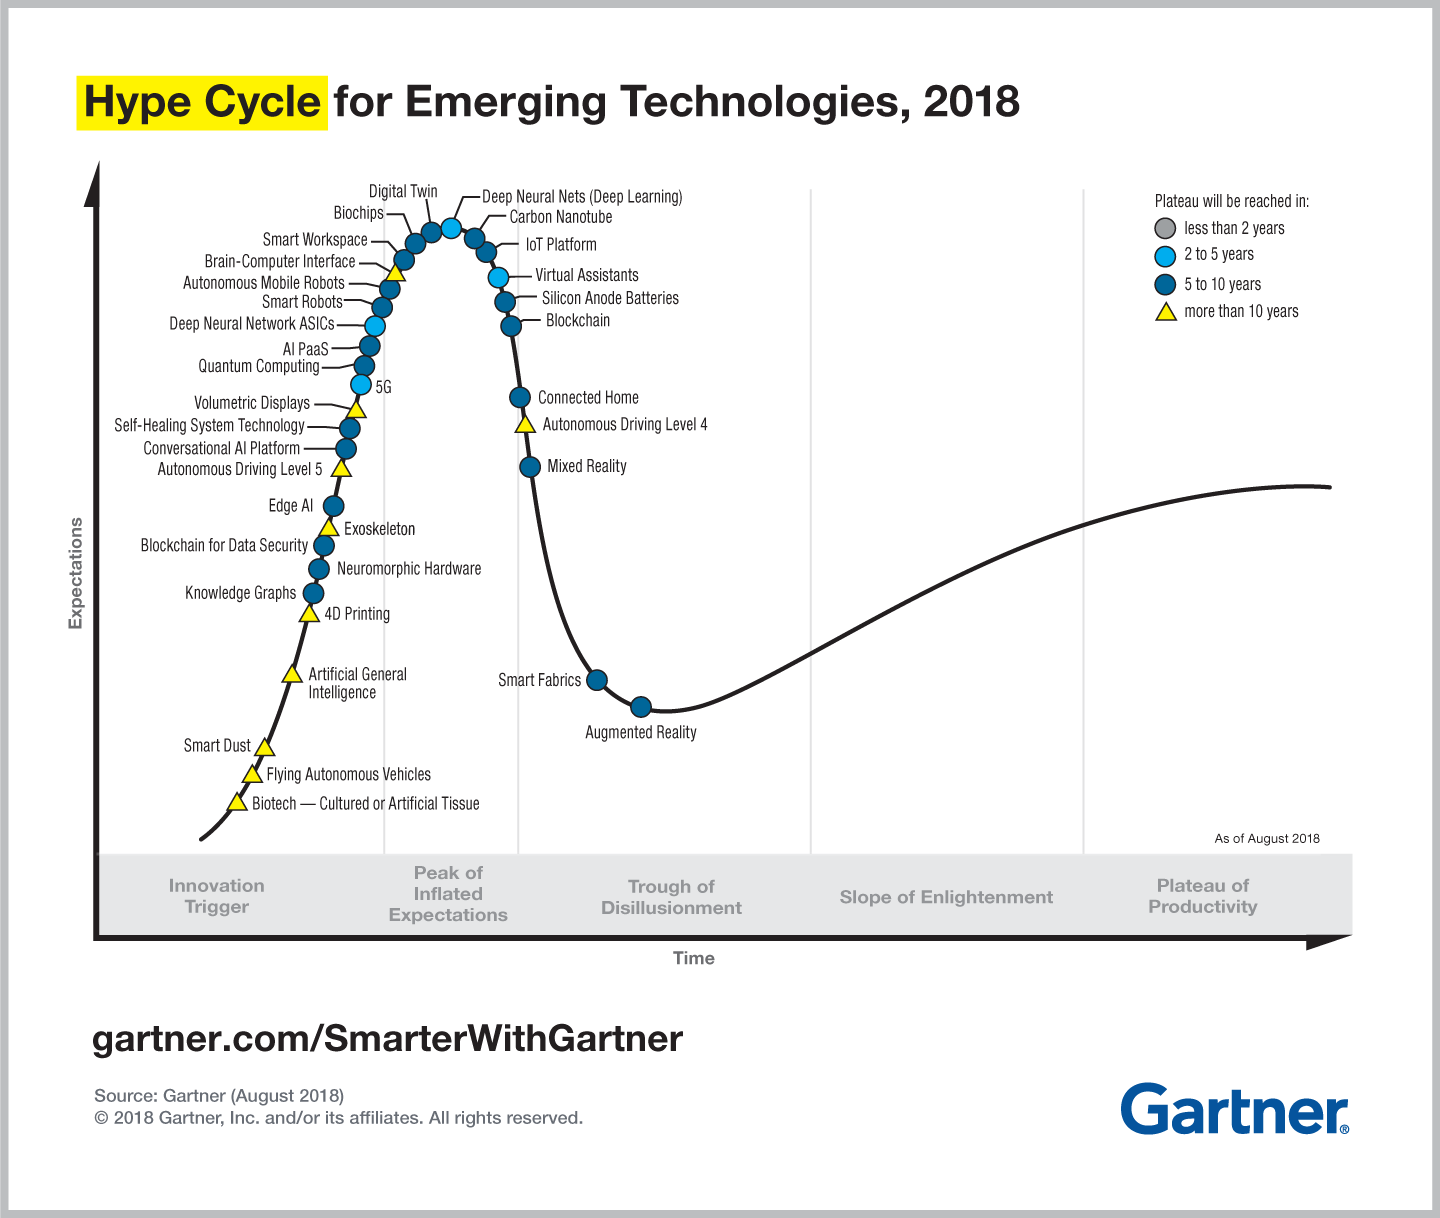
\includegraphics[width=0.7\textwidth]{PR_490866_5_Trends_in_the_Emerging_Tech_Hype_Cycle_2018_Hype_Cycle.png} 
                \caption{Gartner report of emerging technologies 2018}\label{gartner-2018}
            \end{figure}

            It is important to note though that as of 2018, it'll still take more than 10 years to reach a plateau of productivity.
            Although there is no mention about this technology in subsequent reports in the following year, two market revenue forecasts from 2015 until 2022 and 2018 until 2022 show a similar pattern in figure \ref*{statista-revenue}.

            \begin{figure}[h]
                \centering
                \subfloat[\centering \cite{Statista.24052021b}]{{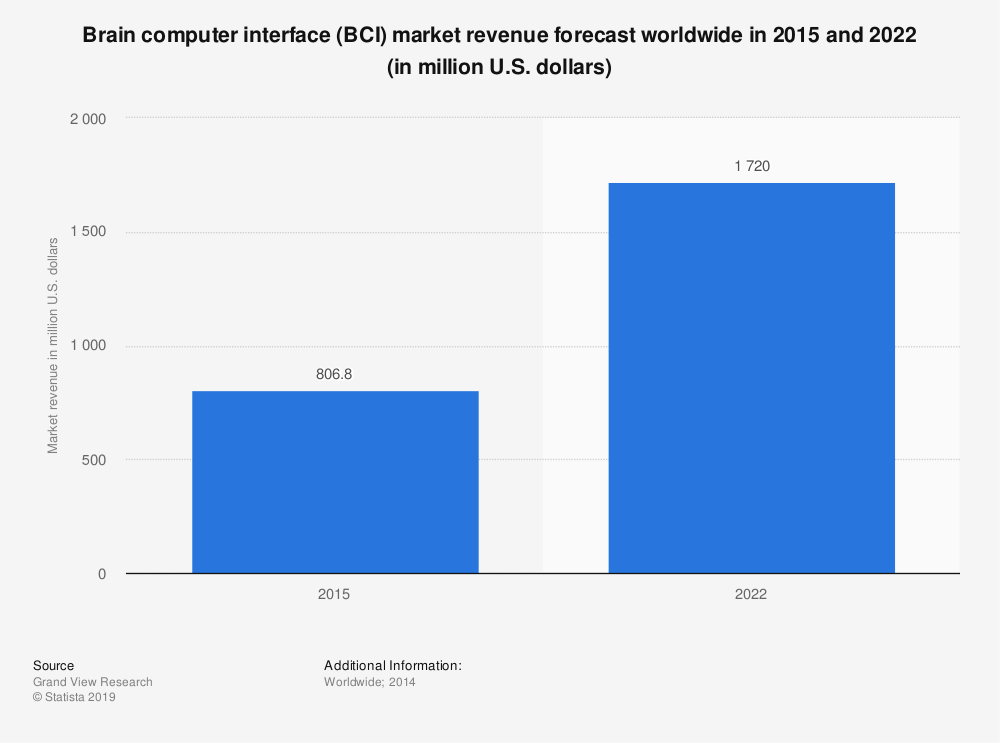
\includegraphics[width=0.49\textwidth]{statistic_id1015039_brain-computer-interface-market-value-worldwide-2015-and-2022.png} }}%
                %\qquad
                \subfloat[\centering \cite{Statista.24052021}]{{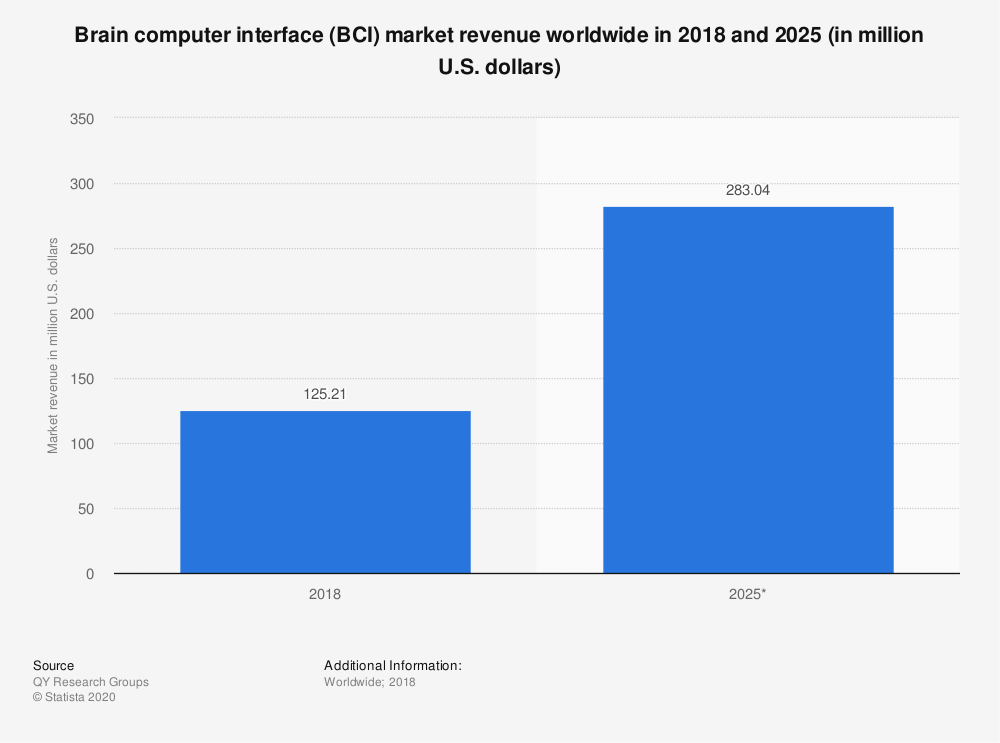
\includegraphics[width=0.49\textwidth]{statistic_id1015013_brain-computer-interface-market-value-worldwide-2018-and-2025.png}}}%
                \caption{Statista revenue forecast as of 2015 and 2018}%
                \label{statista-revenue}
            \end{figure}        

            Essentially the market revenue expectation has been very inflated from 2015 on so that it was corrected downwards in 2018. But although the absolutes growth was projected to only a small fraction, the relative growth potential stayed about the same of doubling within the next seven years. This is very indicative for the technology being overhyped, as Gartner explains: (\cite{Gartner.24052021})

            \medskip
                \emph{A wave of “buzz” builds and the expectations for this innovation rise above the current reality of its capabilities. In some cases, an investment bubble forms, as happened with the web and social media}
            \medskip

            Nevertheless, what this technology sets apart from other featured technologies is the fact that is has been around for a few decades and has been continously researched upon. A strong indicator is the amount of organizations and conferences held about this entire discipline, as can be seen in section \ref*{related-work}. The fact that is has only been on the radar of early adopters and tech-enthusiasts in conjuction with market revenue projections is a strong indicator that this technology has reached a level of maturity which makes a widespread application outside of laboratories somewhat feasible.

            The latest \textit{2020 Gartner Hype Cycle} report shows already the enhanced version of bidirectional BCIs (titled \textit{"2-Way Brain Machine Interface"}) on the slope of innovation:

            \begin{figure}[h]     % h=here, t=top, b=bottom, p=page
                \centering
                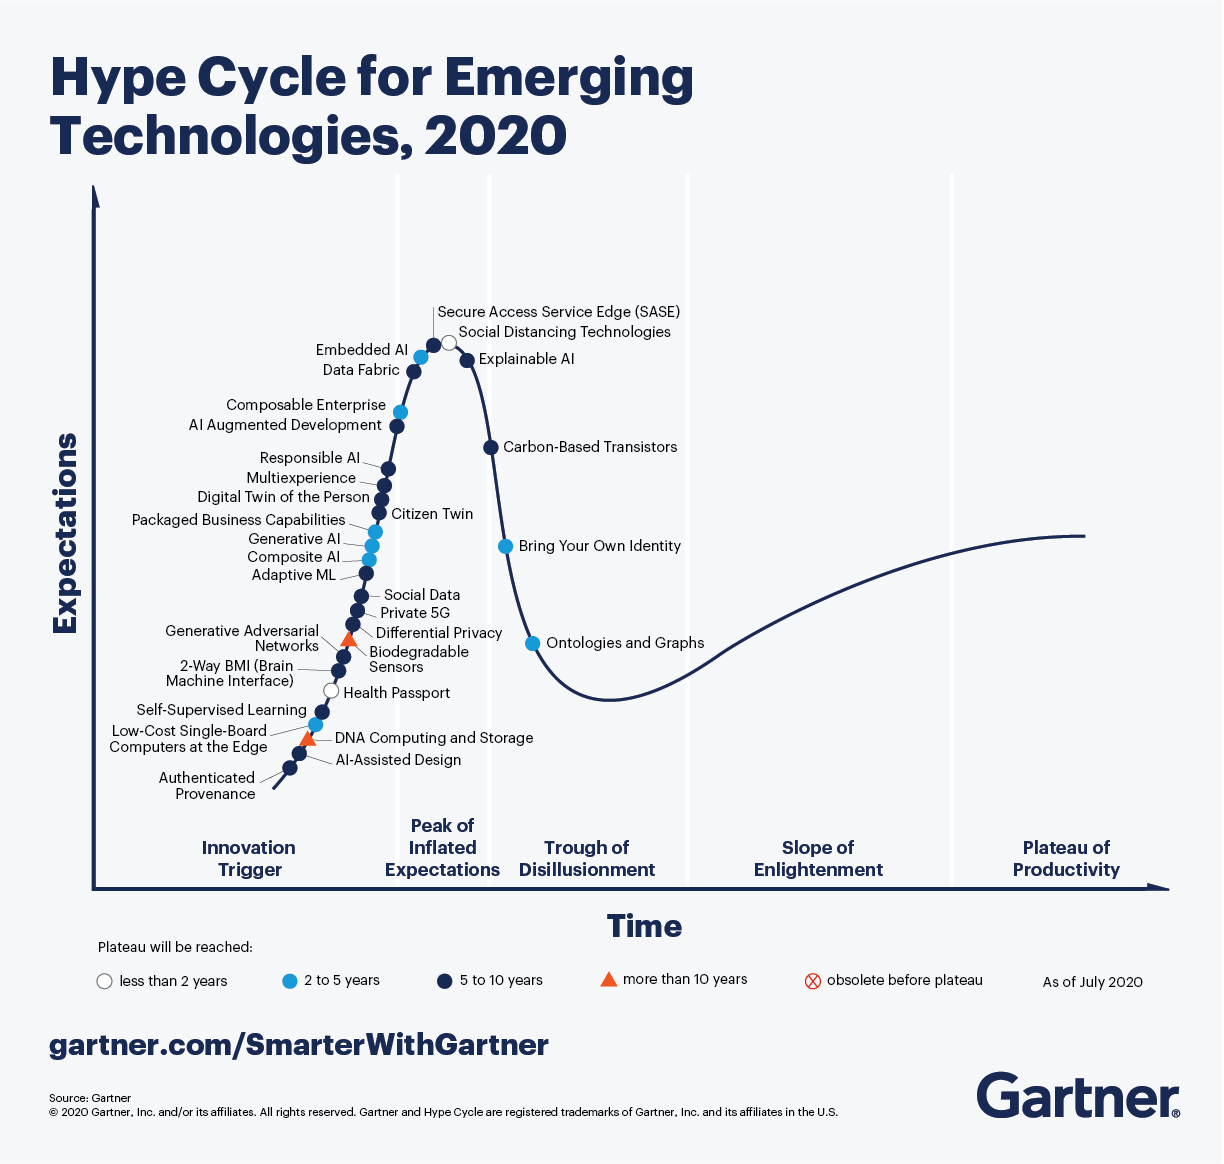
\includegraphics[width=0.8\textwidth]{gartner-hc-emerging-2020.png} 
                \caption{Gartner report of emerging technologies 2020}\label{gartner-2020}
            \end{figure}

            All in all, there are strong indicators that the technology gained traction over the last few years and could be considered a worthwile investment if approached with care.

        \section{Brain-Computer-Interfaces}\label{intro-bci}

            In this section a general overview of the working principle of these interfaces will be provided. Since this study is aimed at computer science and HCI\footnote{Human Computer Interaction}, the neuroscience and medical domain will be only covered very briefly.

            First studies began by \cite{Vidal.1973}, who investigated the possibility to use EEG\footnote{Electroencephalogram} waves, which were first recorded by \cite{Berger.1929}, as a way to create a direct interaction between a machine and a human brain. 

            There are three types of BCIs: invasive, partially invasive and non invasive. This depicts the degree of intrusion into the skull and brain tissue. \textit{Invasive} BCIs are electrodes, which are implanted directly into or onto the grey matter of the brain. This can cause long term issues like scars and also degraded singal strength according to \cite{Abdulkader.2015}. 
            Partially invasive BCI however are although located within the skull not in direct contact with the grey matter.
            Non-Invasive BCI are only placed on the head without intrusion of any tissue.
            Due to the direct contact, invasive BCI provide the best resolution of the measured signals. Non-invasive BCI in comparison suffer from signal degradation and deformation of the cranial bone tissue. 
            Therefore partially invasive BCI are a compromise between good signal strength and the risk of medical conditions.
            Another potential advantage of non-invasive BCIs is that these Interfaces could be easier mass-produced and become affordable to consumers. Also they don't require specialized medical knowledge and equipment to operate.

            The way these interfaces work is based on the same principle: A human brain emits electrical signals, which can be picked up.
            According to \cite{Vidal.1973}, they can be described as follows:

            \medskip
            \emph{"Embedded in this sustained "spontaneous" or "ongoing" electrical activity, short, distinctive (0.5-2 sec) waveforms can be found that are evoked, for instance, when a brief sensory message (stimulus) such as a brief illumination of the visual field or a tap on the forearm is received by the subject."}
            \medskip

            Based on the origin within the brain, these can be correlated to certain stimuli, mental and emotional states (\cite{JardimGoncalves.2018}) and according to \cite{Waldert.2016} been used to drive \emph{an external effector or affecting internal body parts and functions.} The external effector is the use case which is being examined in this study.

            Without a BCI, interaction with a computer requires some physical interaction with devices such as keyboards, mouses or gestures on a touch screen. There are mainly two different reasons, why these devices are a constraint to speed and efficiency of HCI. The first reason is a limitation on interaction speed: Although there is no definitive concensus about the speed of thinking, alone being able to type along the spoken word is unattainable for non-professional typists. A professional typist has to be able to type at 180 - 220 WPM\footnote{Words Per Minute} according to \cite{NCRA.25052021}. \cite{ScienceDaily.25052021} made a survey with 168.000 volunteers, where the fastest typists weren't even able to come close to this mark with 120 WPM. Therefore it is safe to assumt that typing in the same speed as thinking is impossible except for rare individuals who devoted a significant time practicing. Secondly: in applications such as games, where reaction time and accuracy is the fundamental element for success or failure, an interaction based on motoric interaction with a physical pointing device has some significant drawbacks like limited accuracy, if the whole chain of wrist movement in conjunction with a mouse is under scrutiny. 

            If a BCI was to replace these types interaction, these constraints could potentially be alleviated and interaction based on physical interaction rendered obsolete. 

        \section{Working principle}\label{working-principle}         

            Before any deeper considerations in regard to the general scope of this study can be made, it is important to understand the working principle of the BCI, which will be used. Although the vendor of the BCI in question does not disclose any details of the inner workings itself, it is safe to assume that the underlying technique used is the so called \textit{Steady State Visually Evoked Potential} - SSVEP in short. \cite{Sokol.1976} provides detailed inside into the topic from a neuroscientific point of view. The general principle however is that any visual stimuli cause a certain pattern of waves within the visual cortex of the brain. These patterns can be used to evaluate if a certain pattern is being seen \textit{and} in fokus of the person. 
            
            \begin{figure}[h]     % h=here, t=top, b=bottom, p=page
                \centering
                
\includegraphics[width=0.8\textwidth]{placeholder.jpg} 
                \caption{How VEP works in principle \todo{citation?}}\label{vep-principle}
            \end{figure}            
            
            This is being done by subsequently feeding the sensor data through a trained neural network. The objects, which are being seen by the person, have been labeled \textit{neurotags} (\cite{NextMind.23112020}) from the vendor of the BCI. These neurotags can provide two different readouts: If it is triggered (i.E. \textit{seen}) and the confidence, which depicts the level of \textit{focus} of the user on the neurotag (\cite{NextMind.18112020}).
            
            \begin{figure}[h]     % h=here, t=top, b=bottom, p=page
                \centering
                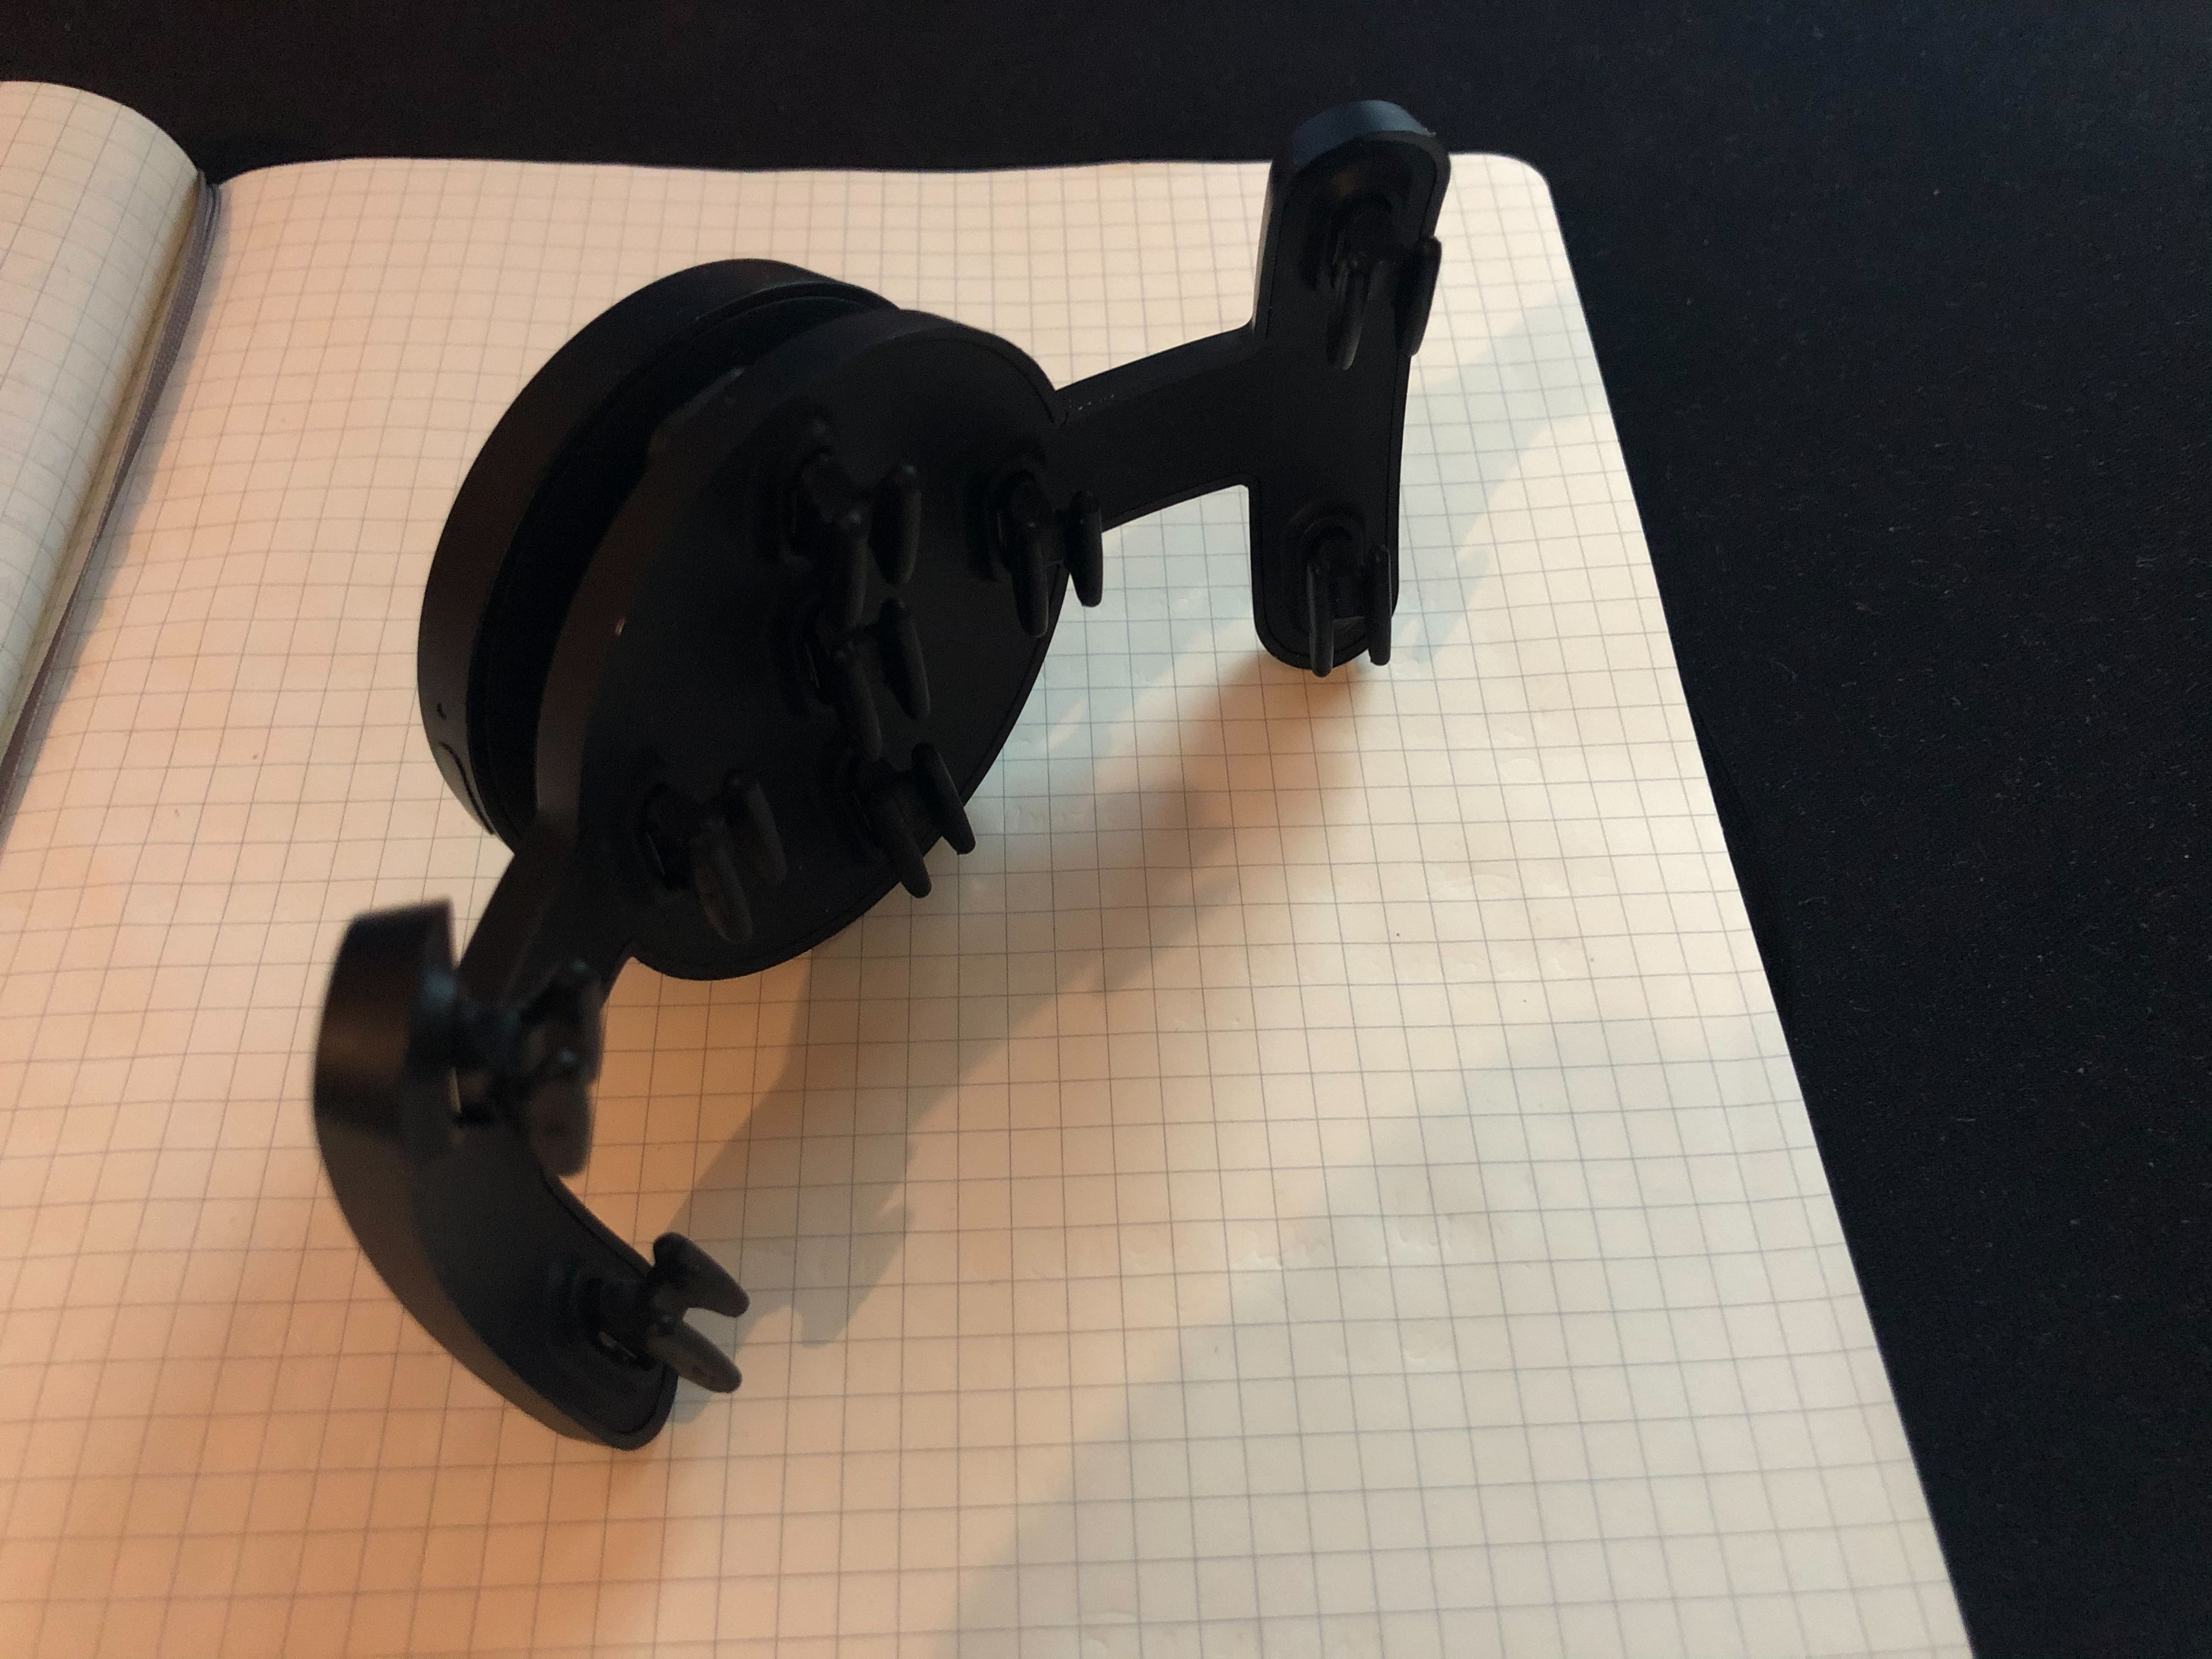
\includegraphics[width=0.8\textwidth]{electrodes-sensor} 
                \caption{Physical layout of the sensor}\label{electrodes-sensor}
            \end{figure}
            
            The physical layout of the sensor is show at figure \ref*{electrodes-sensor}. It has 18 eletrodes, which are arragend in pairs to cover the area, where the visual cortex is located at on the back of the cranium. It is battery driven and communicates via the Bluetooth LowEnergy protocol.

        \section{Related work}\label{related-work}

            As previously mentioned in section \ref*{introduction}, research on BCIs is partitioned between four different domains: \textit{medical engineering, neuroscience, computer science and HCI}. Apart from commercial entities such as \textit{Microsoft} or \textit{IBM} and scientific journals, the majority of the research community is clustered in three organizations: 

            \begin{itemize}
                \item ICBCI (\textit{International Conference of Brain Computer Interfaces}), which is a department of the WASET (\textit{World Academy of Science Engineering and Technology})
                \item EMBS (\textit{Engineering in Medicine and Biology Society}), which is a department of the IEEE
                \item BCI Society, which is an entity of its own
            \end{itemize}

            \medskip

            \emph{There are also research efforts in the east-asian region, according to corresponding tech-sites such as \cite{GlobalTimes.20042021} and \cite{TechwireAsia.24052021} but due to a language barrier, these sources cannot be considered.}

            \medskip

            To narrow the scope, where this research paper is located at, the considerations from section \ref*{use-case-main} are taken into accout. As already established in section \ref*{working-principle}, the sensor used in this study uses SSVEP and is non-invasive in nature. Therefore the general scope of this research is located in the realm of \textit{non-invasive BCI based on SSVEP used for HCI}.

            \medskip

            \cite{Oralhan.2016} and \cite{Resalat.2011} investigated the effects of different twinkle frequencies and duty cycles on the efficiency on precision of SSVEP BCI. They found that a certain combination of these parametres on fact could improve the ITR\footnote{Information Transfer Rate}. \cite{Lee.2016} used a similar approach and found the ideal combination in conjuction with Korean characters.
            \cite{S.M.Abdullah.2014} used a consumer ready BCI by \textit{EMOTIV} to create a \textit{Matrix-Speller} in the Bengali-Language to allow people who have lost the ability to communicate to express themselves again. 
            \cite{Chen.2020} also used a SSVEP BCI to implement a BCI-speller and scrutinized the tradeoff between responsiveness and accuracy.
            \cite{Chen.2020} designed an interface which is operated by a SSVEP BCI to control a robot arm, wich could administer food to disabled people.
            \cite{Soroush.2018} developed a SSVEP BCI which overcomes the necessity for training the sensor to the user who wears it. The prototype reached a similar precision as \textit{trained} interfaces.
            \cite{Gergondet.2015} investigated and selected certain visual stimuli which work best with certain use cases.
            \cite{Merino.2017} made a study, where participants controlled a UAV by using a SSVEP.
            \cite{Peters.2018} used simulated impairments to examine if usage of a SSVEP is still possible with medical conditions which affects speech and ocular impairments.

            Although not strictly within the SSVEP domain, the study by \cite{Beveridge.2017} showed very promising results by not using visual stimuli but mechanical ones, where he had teenagers playing a racing videogame with the aid of mechanical stimuli.

            There is a massive ongoing research effort to make the life of people who are suffering under ALS\footnote{Amyotrophic lateral sclerosis} better and improve their ability to communiate normally, by using SSVEP, a hybrid between an SSVEP and P300\footnote{An Event Related Potential (ERP) BCI} or purely P300 based BCI. A significant number of relevant studies has been published in the BCI Society Journal: \cite{Sugata.2016}, \cite{Holz.2015}, \cite{Speier.2017}, \cite{Geronimo.2017}, \cite{Speier.2018}, \cite{Mowla.2017}, \cite{Huggins.2016}. All these studies aimed to provide a better understanding and performance of using BCI on people with medical conditions, which cause serious physical impairments.

        \section{Establishing a use-case}\label{use-case-main}

            Establishing a use-case in the context of this study is a pivotal point hence this section will be split up into several sections: 

            \begin{enumerate}
                \item General considerations
                \item Deduction of the core points of this study
                \item Evaluating the constraints of a participatory study
                \item Deduction of use-case
                \item Conclusion into hypothesis and use-case
            \end{enumerate}

            \subsection{General considerations}

                The first step in conceiving any potential way of using such a device is to evaluate the way any user could interact with a BCI with a computer. According to \cite[4.13]{Buxton.2010} the way users interact with a device require an agent of control i.e. a hand, what is being sensed by the device (position, motion or pressure) and the number of dimesions being sensed (1, 2, 3). This results in a different input taxonomy for any given device. However, a BCI does not have either of these parametres, since the interaction does not require physical interaction. Hence a classification by means of using a taxonomy cannot be achieved. Where the interactions of BCIs can be compared to those classified by taxonomies is by the way they functions they apply in relation to a user interface.

                The API\footnote{Application Programming Interface} endpoints of the NextMind sensor offers two different modes of interaction. These are explained in the SDK\footnote{Software Development Kit} of the sensor in detail: \cite{NextMind.18112020}.
                They are depcited as \textit{tracking resuls} with a \textit{hit} property and a \textit{confidence} metric. Where hit is a two state interaction: the neurotag is being seen by the user and subsequently recognized by the sensor and its backend or it is not. The confidence property depicts the attention which the user is paying to the \textit{neurotag}. This is a continuous decimal value between 0 and 1.
                The fact that these types of interaction are based on neural activity raises the question if a pure mapping of continuous and discrete input modalities to established interfaces would be beneficial to the user experience. Under the reasonable assumption that without any training the metric \textit{focus} can only be deliberately controlled on a very coarse level, the necessary sensitiveness required for modern GUIs\footnote{Graphical User Interface} can not be achieved with this particular sensor. The remaining two state property, which can be utilized to select or deselect certain objects also only allows for limited interaction. However, these neurotags can be placed in arbitrary places. Although a \textit{toggle}-like behavior is not mentioned explicitly, it might be possible to de-select any activated neurotag when the \textit{focus} property falls under a certain value.

            \subsection{Corepoints of this study}\label{corepoints}

                Based on the previous reasoning, the following questions can be raised in regard to the feasibility of any interface which could potententially be conceived with this technology:

                \begin{enumerate}
                    \item How fast is the perceived and measured reaction time of these neurotags?
                    \item What is the minimum size the neurotags have to have in order to be recognizable?
                    \item Is the interface usable for brains of all ages or do gerontological effects have an effect on usability?
                    \item Do certain medical conditions (i.e. attentiveness disorder) have an impact on the usability?
                    \item How fast can a user switch between neurotags?
                    \item Is a BCI controlled GUI intuitive to use?
                    \item Does a personal affinity to technology have an influence on the perceived difficulty of interaction?
                \end{enumerate}

                These questions can be clustered into two groups: \textit{neurological} and \textit{interaction}. But all these considerations open up a vast space of potential cases, hence the priority is to examine wheter these interfaces are generally usable by the majority of users and if these interfaces are intuitive to use. Out of this list only the points 1, 2, 3, 5, 6 and 7 can be applied to a general audience. Considered the possible interactions with the \textit{Nextmind} sensor, a study which focusses on the neurological domain makes more sense in the context. \todo{Revisit reasoning.} This leaves the points 3 and 5. Although these are two different topics, the setup of the experiment itself will show that in fact number 5 can be examined along the way as well, which wil be discussed in section \todo{Add ref + revisit argumentation.}

            \subsection{Constraints of a participatory study}
            
                Although this study won't use the \textit{AttrakDiff} survey, which was designed by \cite{Hassenzahl.30092020}, it is still worth considering how a potential use-case might peform in the context of an \textit{AttrakDiff}. The reasoning is that a survey, which is entirely construted to serve the purpose of producing results in favour of the study, might be harder to grasph for the participants in the experiment. The reason being that an interaction purely for the sake of interacting with something does not provide an incentive for the user to do so. As a consequence, the results which are produced by the participants, might be skewed due to a lacking frame of reference.

                \begin{figure}[h]     % h=here, t=top, b=bottom, p=page
                    \centering
                    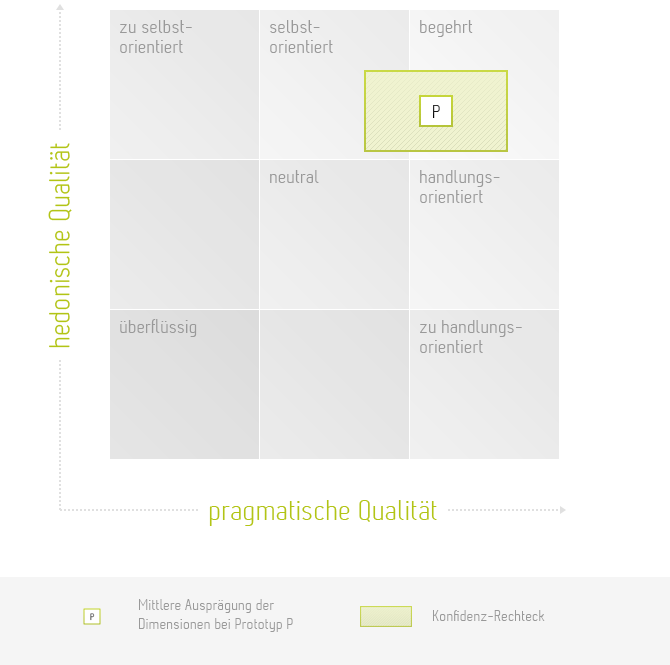
\includegraphics[width=0.8\textwidth]{einzelauswertung_de.png} 
                    \caption{\todo{MAKE ENGLISH} AttrakDiff results for a given interaction model, Source: \cite{Hassenzahl.30092020}}\label{AttrakDiff}
                \end{figure}

                Figure \ref*{AttrakDiff} shows two axes which depict the hedonistic quality of an interaction, which is a metric of pleasure and the pragmatic quality which depicts a metric of \textit{ease of use} or \textit{technical quality}. Even without any deeper knowledge it is safe to assume that it is preferential for the interaction to be located in the upper right corner, since this makes it \textit{"desireable"} instead of \textit{"unnesessary"}. Given that, it is certain that any interaction needs a way to facilitate pleasure in the user.

            \subsection{Deduction of use-case}\label{use-case}

                Concluding the two parametres \textit{frame of reference} and \textit{facilitation of pleasure} into a coherent picture, it can be inferred that the experiment has to be set up in way that gives the participants a familiar use case which facilitates positive feedback. 

                As already established, this study will examine gerontological effects in the context of an interaction. Therefore the age of participants will very likely vary to a wide degree, what necessitates a use case which is common to all age groups alike. Because people above a certain age did not grow up with computers, an experiment which relies heavily on the usage of computer as main point of interaction is very likely not a good choice due to the difference in proficiency. One example where both these criteria are met is a remote control for a television. Although nowadays there are computers involved, the interaction hasn't really changed in the last decades on a general level.

                Nevertheless the working principle of the BCI is a visible flashing pattern, as established in section \ref*{working-principle}. Therefore the representation of some kind of GUI on a display is still necessary. Since VR goggles provide better isolation from external visual stimuli, the representation within a VR application was chosen. 

                \medskip

            \subsection{Concluding hypothesis and use-case}\label{hypothesis}
            
                Section \ref*{corepoints} established that age is the first parameter to examine in this context, therefore the fundamental research hypothesis can be defined as follows:

                \medskip
                \emph{"Age does not have a detrimental effect on the ability to use a non-invasive BCI based on VEP technology."}
                \medskip

                In Section \ref*{use-case} the fundamental reasoning behind the use case, which provides the necessary framework for this study was established:

                \medskip
                \emph{A GUI which represents a tv remote control will be presented to the participants within a VR environment.}
                \medskip

        \section{Beyond the scope}\label{beyond}

            The case in this study is fairly limited in the realm of BCI. Section \ref*{related-work} already briefly mentioned that the general research on BCI has several fascinating topics to explore. This section aims to broad the horizon on the realm of BCI technology.

            \paragraph{Picture synthesis}

                In 2019 \cite{Rashkov.2019} published a paper which outlined the reconstruction of images seen by individuals by means of a BCI. They used a 128-channel EEG cap to record brainactivity in a 1...35Hz bandwidth while being shown videos of different subjects. The signals were treated with a PCA\footnote{Principal Component Analysis} to create a 20-dimensional feature vector which is feeded into a classification model, which yields the results:

                \begin{figure}[h]     % h=here, t=top, b=bottom, p=page
                    \centering
                    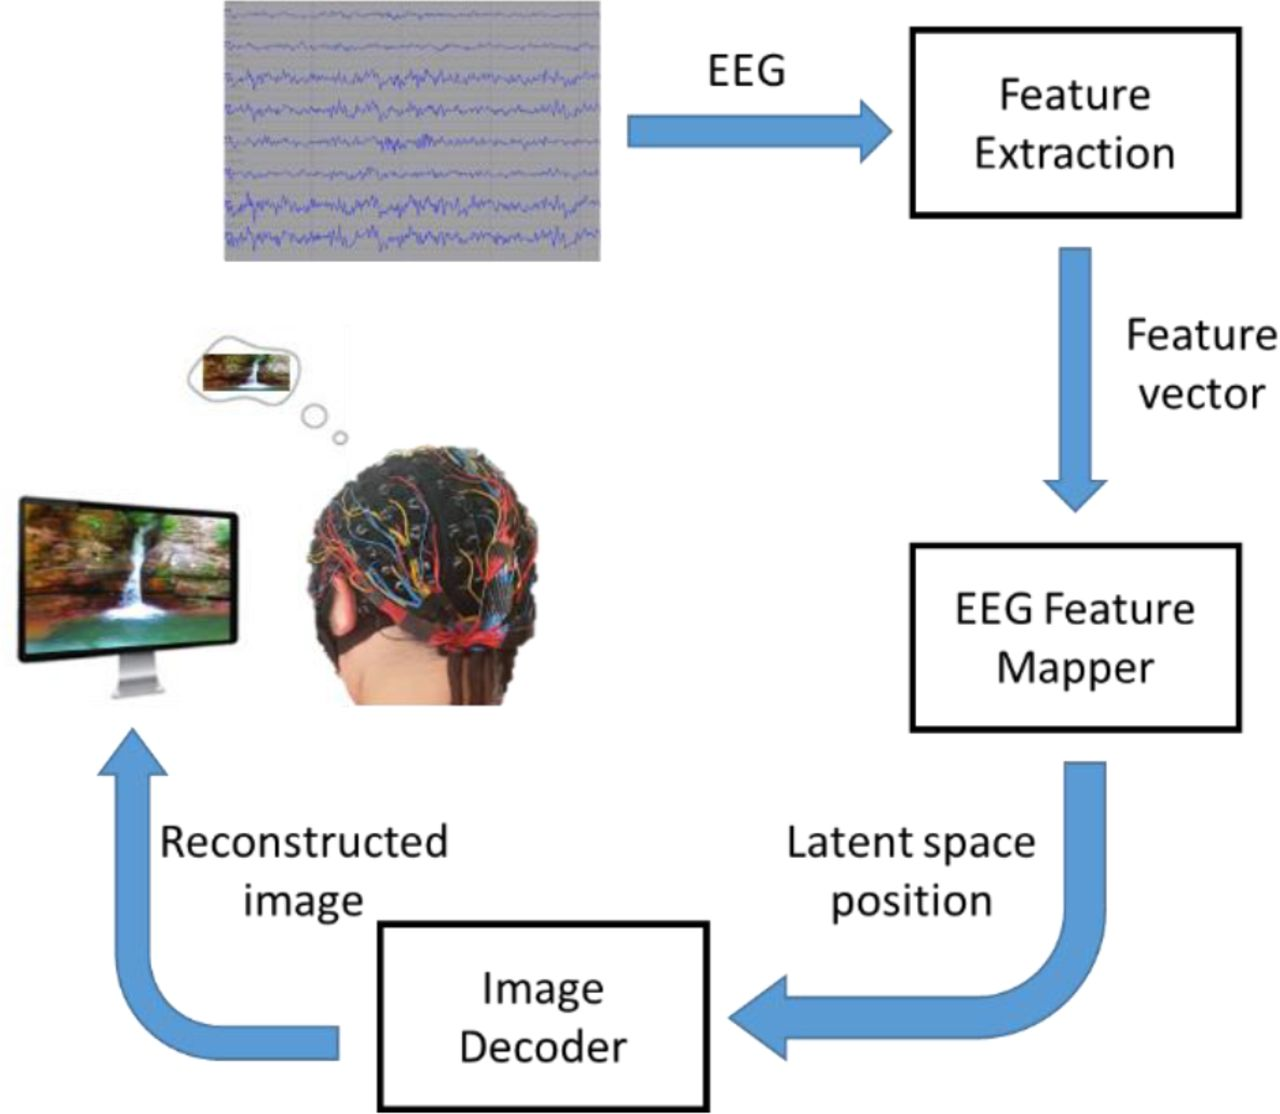
\includegraphics[width=0.8\textwidth]{F2.large.jpg} 
                    \caption{General scheme of neurofeedback model, Source: \cite{Rashkov.2019}}\label{image-synthesis}
                \end{figure}

                \cite{Oneill.14112019} wrote a good summarized article about the paper alongside results and a video which features a demonstration. On the other hand \cite{HernandezCarmona.2019} used a similar approach to enhance grasping of robotic arms by means of deciding on the correct technique to grasp based on image reconstruction from a BCI.

            \paragraph{Controlling vessels, aircraft and spacecraft}
                
                Since BCI like the P300 have been used as neuroprosthetics for physically impaired people, there are efforts made to study a broader application of BCI to control machines or vessels. \cite[]{Choi.2018} published a study, where  invasive BCIs for direct control of machines were examined. They came to the conclusion that this is very much possible but requires several advancements to gain really high quality data for fine-motoric movements. This also requires that electrodes have to be implanted deep inside the brain in order to gain high resolution results.

                \cite[]{WilliamKucinski.2018} published and article on the SAE News homepage, describing a report published by the DARPA where an individual was able to control three warplanes in a simulator. The novelty in this research was also the feedback given to the individual, thereby posing a bidirectional BCI. As of Q2 2021, this article is no longer available on the DARPA homepage but several other news organizations wrote about this: \cite[]{Stockton.03052015}, \cite[]{Blair.2018} and \cite[]{Tucker.09062018}. Since the DARPA is well known for being decades ahead with their research, it is very well feasible outlook to have BCIs in the future, which allows for control of not only aircraft but also ships and spacecraft.

            \paragraph{Improving human learning rate and augmenting system performance}

                In an article published by the Journal of neuroscience methods by \cite[]{Miranda.2015} the efforts by the DARPA\footnote{Defense Advanced Research Projects Agency}, which is a US federal agency to advance technology for defensive efforts, were outlined. These grouped into prosthetics and rehabilitation as well as efforts to improve human training and performance. The latter has fascinating research on Improving the learning rate of the human brain:

                \medskip
                \emph{The Narrative Networks (N2) program is developing new techniques to quantify the effect of narratives on human cognition and behavior, including initial development of a closed-loop BCI system that adapts a narrative in response to a listener's EEG signals. Such a system would have numerous applications to training and human performance domains.}\cite[]{Miranda.2015}
                \medskip

                Further applications were the integration of a \textit{Human-in-the-loop}, scenario, where intelligence analysis and threat warning. A 10-fold improvement in analysis throughput was achieved in the former case. In the latter case of threat detection the incorporation of a BCI-enabled human increased the probability of threat detection to 91\% compared to 53\% detection rate solely relying on computer vision.

            \paragraph{Transferring thoughts over the internet}

                A paper published by \cite[]{Martins.2019} outlined the possibility of using nanotechnology to insert sensors to every single neuron and synapse in the human brain to have a real time stream from the within the human brain with a resolution down to a single neuron. This would allow for every human having a digital twin of himself in the cloud, having access to the whole repository of human knowledge withoug timedelay and even share experiences, thoughts and memories with other people.

                \begin{figure}[h]     % h=here, t=top, b=bottom, p=page
                    \centering
                    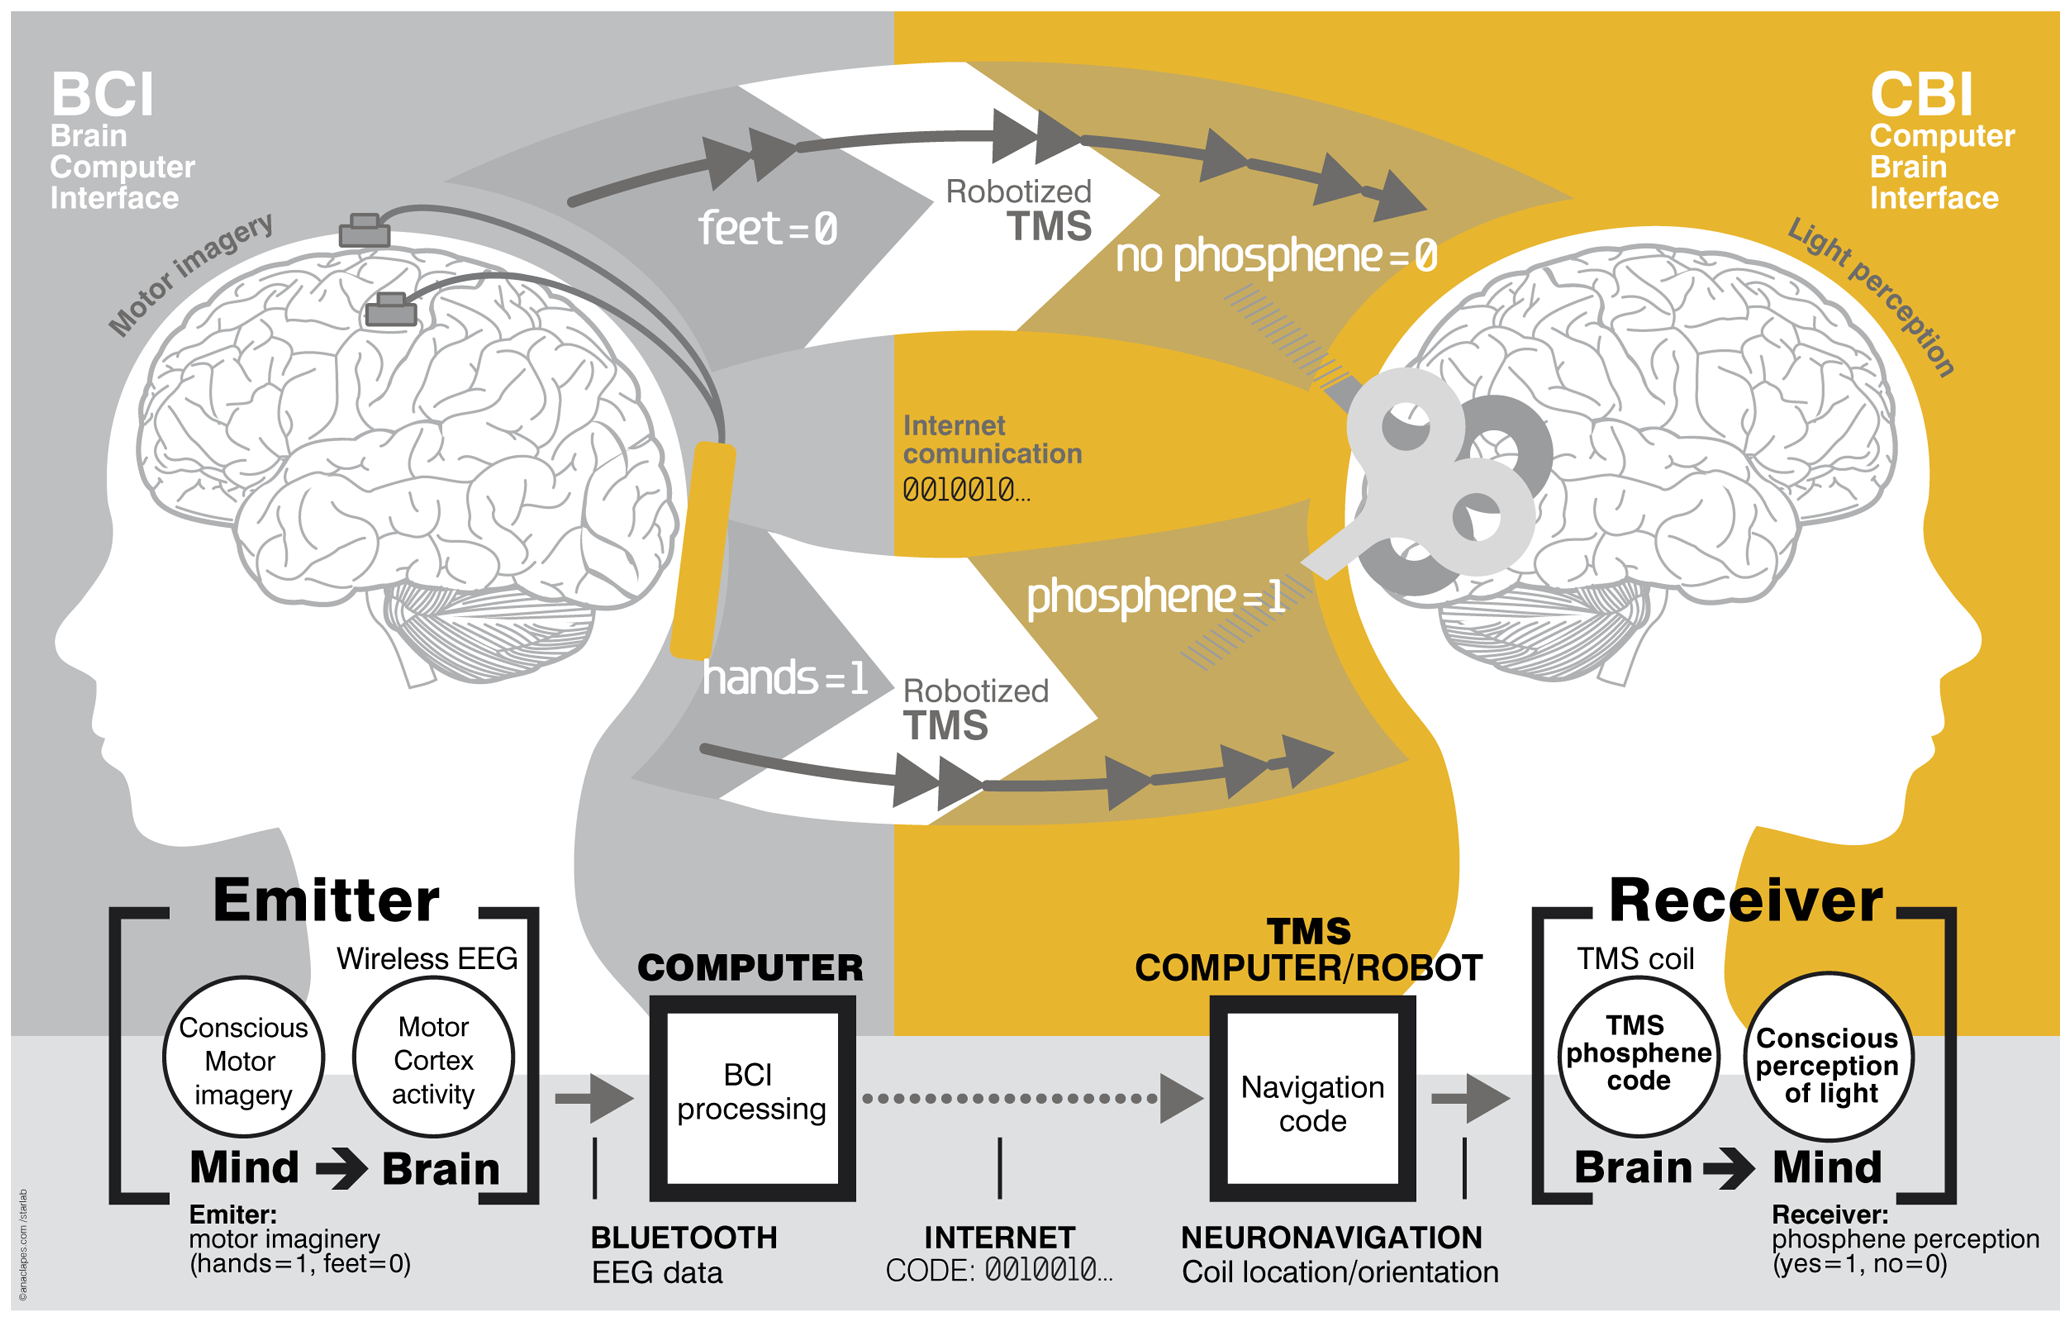
\includegraphics[width=0.8\textwidth]{pone.0105225.g001.PNG_L.png} 
                    \caption{B2B communication signal chain, Source: \cite{Grau.2014}}\label{b2b-chain}
                \end{figure}    

                A little less futuristic is a study published by ABC News: \cite[]{Lee.2016} and outlined in figure \ref*{b2b-chain}. In this case for the first time in human history, conscious communication from one brain to the other without the involvement of sensory or motoric stimuli was achieved. This is called a B2B or Brain-to-Brain communication. The according paper was written by \cite[]{Grau.2014}. In this case two humans exchanged the greetings \textit{Hola} and \textit{Ciao} over the internet from India to France.

            \paragraph{Data privacy}

                With the latest innovation in the field of BCI and BMI a new concern arises along with them: privacy. \cite[]{Greenberg.2019} published a paper, where she outlined the current status and outlook on data privacy in regard to brain data, where the juristictions of the EU, United States and Canda were compared with their different approaches:

                \medskip
                \emph{In relation to the governance of personal data in the private sector, the United States adopts a self-regulatory mechanism, while the European Union assumes a rights-based approach, with Canada's position being intermediate to the two extremes.}, \cite{Greenberg.2019}
                \medskip

                She concludes that \emph{As BMIs enter the marketplace, legal and ethical questions pertaining to brain data privacy are certain to arise}\cite[43]{Greenberg.2019} and makes policy recommendations to be implented in order to guarantee privacy. These recommendations outline a \textit{privacy by design}, improvement of transparency and general sharpening of existing policies to better suit the requirements of brain data applications.

        \section{EEG acquisition devices}

            Concluding section \ref*{intro-bci} and \ref*{beyond}, it is reasonable to talk about some technical implications of BCIs and their limitations. In technical terms, these are EEG acquisition devices from the medical domain and only gather EEG brainwaves from certain regions of the brain. The placement of the electrodes on the skull determines which domain of brain activity will be recorded. 

            There is a great variety of these different EEG acquisition devices on the market. Ranging from consumer-grade cheaply and readily available sensors which cost a few hundred Euros up to medical grade devices. According to \cite{Zerafa.2018} the difference in price and quality are mainly determined by the factors amplifiers, electrode type and count and transmission technique, which could be wired or wireless.

            Since these sensors measure electrical potentials, the actual resolution of the electrodes and amplifiers ist the single most influental parameter governing quality. \cite{Zerafa.2018} used the SNR\footnote{Signal to Noise Ratio} of different sensors to compare them to one another, because quality in electrical measurements is best compared using the SNR value of each measurement:

            \begin{figure}[h]     % h=here, t=top, b=bottom, p=page
                \centering
                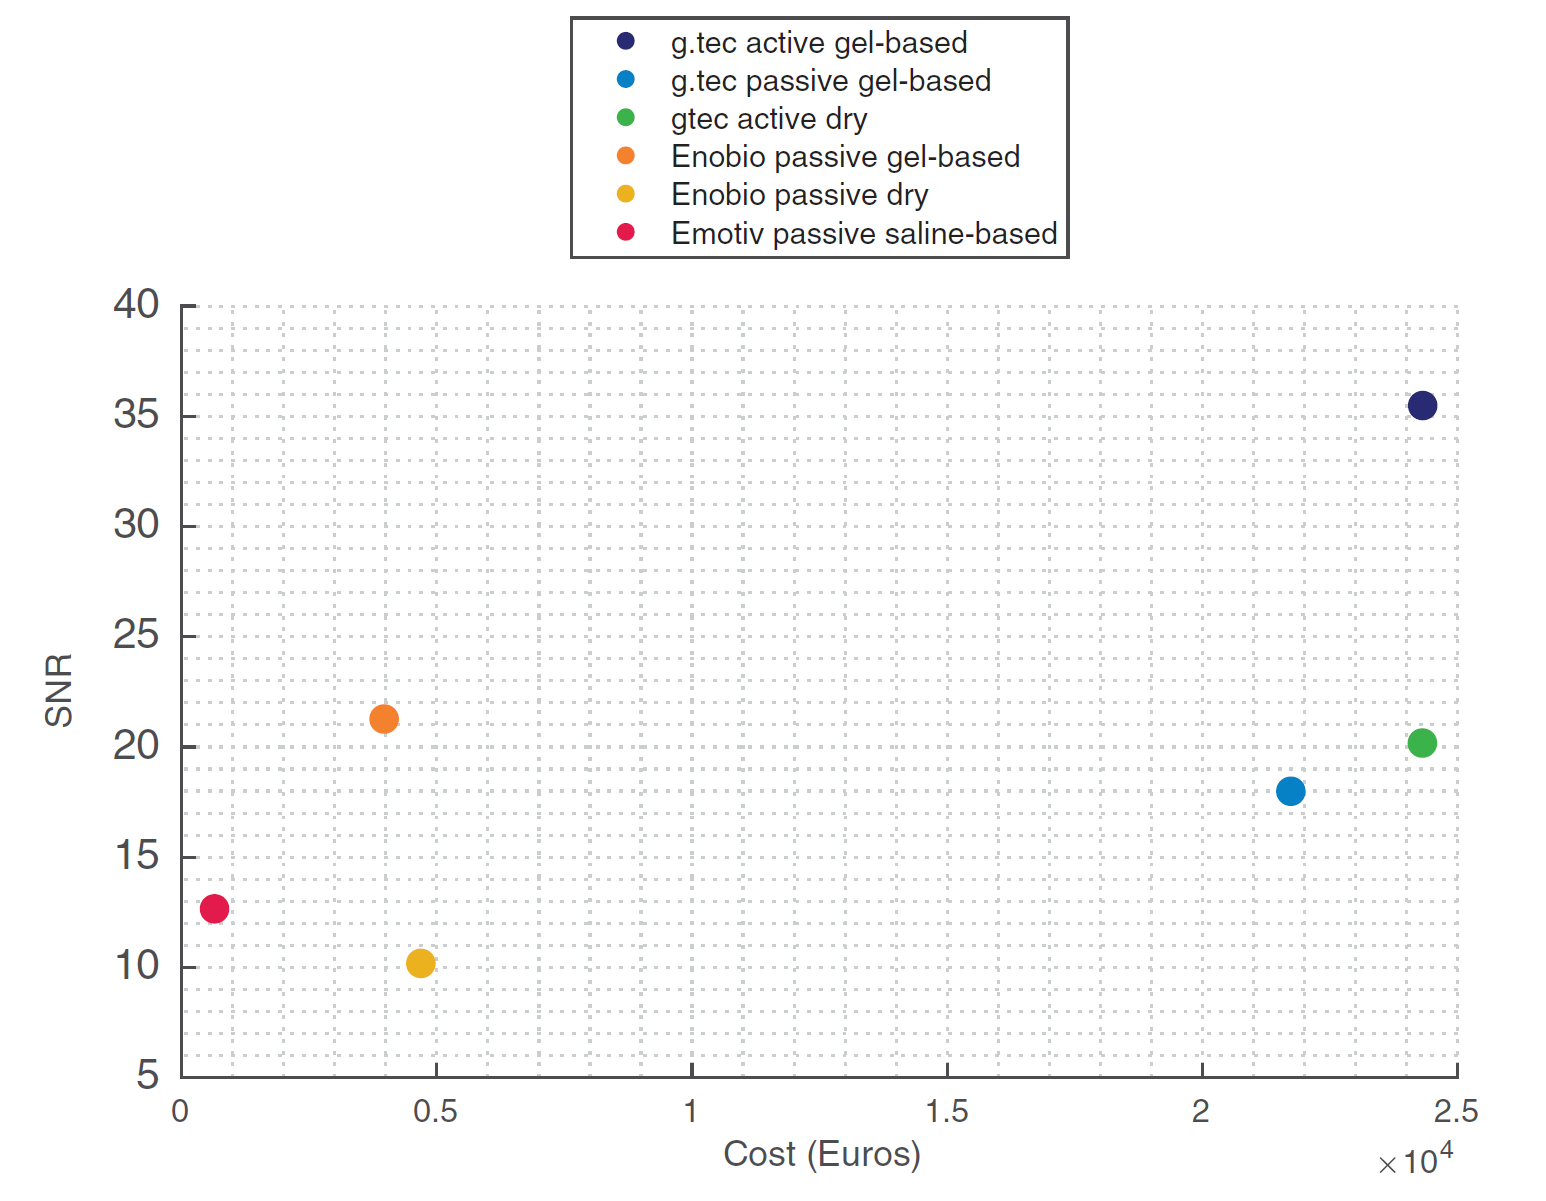
\includegraphics[width=0.8\textwidth]{eur-vs-snr.PNG} 
                \caption{SNR plotted against price, Source: \cite{Zerafa.2018}}\label{snr-eur}
            \end{figure}              
                
            Figure \ref{snr-eur} shows the picture that \textit{cheaper} sensors tend to have a worse SNR than more expensive ones with one exception which performed better. However, the cheaper sensors were perceived more comfortable and their set-up time was significantly less compared to fully fledged medical devices, which made them the better choice for experimenting and rapid prototyping. Also the expensive sensors required special treatment with gels and saline solutions, which wasn't necessary on the dry-electrode setup of the cheaper sensors. The conclusion of \cite{Zerafa.2018} was that either of those two caterogories have their advantages in their own domain and there is no \textit{best choice}.

            \medskip

            \todo{Check if paper can be quoted like that.}

    \chapter{Survey Framework}\label{survey-framework}

        Before any survey can be designed, certain considerations like sample size, population ... \todo{ref to döring/bortz for details}
        have to be taken into account. Also depending on the desired outcome of the survey, the questionnaire has to be defined.

        \section{Considerations}\label{considerations}

            The primary goal of the survey is to find empirical evidence that age does not affect the ability to use a BCI. In order to exclude certain parametres, which might cause an unwanted effect, potential disturbance parametres have to be identified and discussed:

            \begin{itemize}
                \item Age
                \item Gender
                \item Quality of the sensor readings
                \item Motion Sickness
                \item User wears glasses
                \item Cognitive impairments
                \item Medication known to affect EEG readings
            \end{itemize}

            Furthermore participants of the study should disclose if they had previous or ongoing conditions of seizures or epilepsy, especially in case of light or flashing related cases.

            Apart from the demographic parametres of age and gender, the other factors have to be considered to prevent potential malformed data. Firstly, a condition which causes a detrimental effect on the ability to see and identify patterns might have a dampening effect for the visual cortex to create the required brain waves. However, the physical layout of the VR goggles used allow for prescription glasses to be worn. Hence this is not a concern in the context of this study. Secondly, when working with VR goggles, there is always the possibility of motion sickness involved. On the other side: this will unlikely have a negative effect since the experiments will be static. There won't be any movement from either the user itself within the environment nor the GUI involved, which removes the prevalent reason for motion sickenss according to \cite{Golding.2006}.
            Lastly the readings of the sensor will very likely be different for each experiment. Since the sensor provides quality readings, these will be considered in the data evaluation. Nevertheless, there will be a questionnaire provided which will ask the user after experiment if he experienced any of these effects to have a possible explanation for potential outliers.

            \medskip

            Under the assumption that gender has no effect on the study, because the brain of men and women is at least structurally identical. Therefore age is the only parameter which is the variable in this study. To put the results into context, the survey participants will be clustered by age into different groups.

        \section{Design of experiment}\label{doe}

            The solid proof that the hypothesis holds true or not can not be made based on looking at diagrams and educated guesses. Hence the need for design of experiment to provide a numerical framework which defines threshholds and quantities to make results reproductable. This section is based on the theoretical framework which es described in \cite[87ff]{Siebertz.2017} under the considerations in the previous section.
            There are two main parametres to consider, when it comes to the DoE\footnote{Design of Experiment}: 
            
            \begin{itemize}
                \item How many samples are necessary to reliably prove that the hypothesis holds true?
                \item Where is the threshold which determines whether an effect is significant or not?
            \end{itemize}

            In the context of DoE the former is often depicted as $\beta$ and the latter as $\alpha$.

            \paragraph{Parameter alpha - $\alpha$:} Alpha is the governing parameter, which decides how big the risk in a given sample size is that the hypothesis is wrong and therefore falsified. Since the hypothesis can be either true or false, the probability that it is wrong decreases with the number of samples taken in a binomial fashion \cite[103]{Siebertz.2017}. That means in this case that the likelihood $p$ of a participant to be above or below the threshhold, which is discussed in section \ref*{operationalization}, is not determined by age. According to \cite[110]{Siebertz.2017} common values for alpha tend to be chosen such that the probability of a falsified hypothesis is at 1\%, 5\% and 10\%. Where a smaller value means a more strict threshhold. To account for the explorative character of this study the value of 5\% is chosen. Therefore the susceptibility for unaccounted side-effects is reduced and the total number of participants is still not unfeasibly large.

            \paragraph{Parameter beta - $\beta$:} This parameter depicts how effective a potential effect is in a given sample size. The likelihood of a significant effect not being recognized decreases with an increasing number of samples, since it becomes increasingly unlikely that a systematic effect affects the samples always in a way which makes it undiscoverable.
            Table \todo{ref table} shows that with an increasing number of samples, given the determined alpha value, the likelihood decreases rapidly:

            \medskip
            \todo{Create table here}
            \medskip

        \section{Information Transfer Rate}\label{itr}

            After establishing the necessary framework for the survey and how the results have to be interpreted in order to draw a meaningful conclusion, the underlying metric to examine and compare the peformance of the individual subjects in the experiment has to be defined. The most widely adopted metric is the \textit{Information Transfer Rate} or \textit{ITR} in short, according to \cite[1]{Yuan.2013}. This metric was conceived by \cite{Wolpaw.1998} and depicts the bits/symbol:

            \begin{equation}\label{itr-basic}
               B = log_{2} N + P log_{2} P + (1-P) log_{2} [(1-P)/(N-1)]
            \end{equation}

            Where $N$ is the total number of choices for a user to choose from and $P$ is the probability that a desired or required choice in the experiment will be selected, therefore posing also a metric of accuracy. In the context of this study a symbol is equivalent to a single \textit{choice} on the remote control (see Section \ref*{use-case}). However, \cite[4]{Yuan.2013} summarized certain contraints which have to be met, in order to ensure the applicability of this formula:

            \begin{enumerate}
                \item BCI Systems are memory-less and stable discrete transmission channels.
                \item All the output commands are equally likely to be selected $(p(\omega_{i})=1/N)$
                \item The classification accuracy is the same for all the target symbols $(p(y_{i}\vert x_{i}) = p(y_{j}\vert x_{j}))$
                \item The classification error is equally distributed among all the remaining symbols $(p(y_{j}\vert x_{i})_{j \neq i} = (1-p(y_{i}\vert x_{i})/(N-1))$
            \end{enumerate}

            Where (1) is in the scope of this study solely determined by the choice of the interface and (2) solely on the implementation of the experiment. However (3) and (4) would be also considered solely depending on the implementation of the experiment. But since this might be influenced by the performance of the individual participant, there is a possibility of side effects like visual impairments resulting in varying performances when the target symbols are spatially distributed. Nevertheless in line with section \ref*{considerations}, these considerations will be disregarded for the purpose of this study.

            Going into detail regarding (1), it has to be elaborated, why the used sensor is within the set constraints. These are: synchronism, bijectivity regarding the mapping of available symbols and possible selections, no memory, lack of error correction and prediction and no goal directed behavior.

            \paragraph{Synchronism} A BCI works \textit{synchroneous}, when the time which passes from the presentation of a cue to the user until the symbol has been confirmed or erroneously chosen is solely determined by the system itself. A BCI might be considered \textit{asynchroneous} if there are measures in place to artificially increase the response time. 

            \begin{figure}[h]     % h=here, t=top, b=bottom, p=page
                \centering
                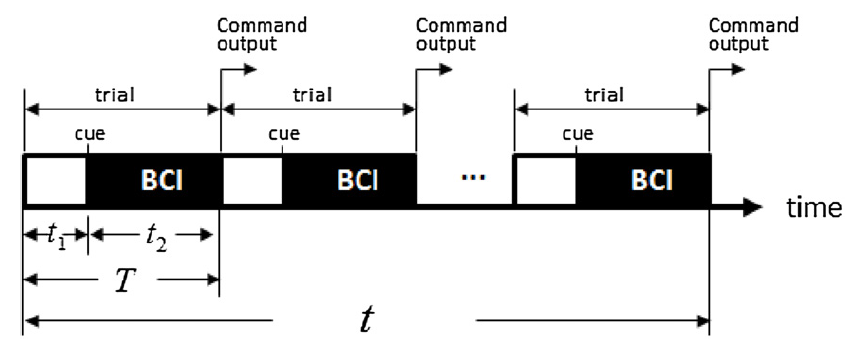
\includegraphics[width=0.8\textwidth]{timingBCI.PNG} 
                \caption{Timing of symbol recognition and activation \todo{/ create own graphic}}\label{itr-timing}
            \end{figure}

            \paragraph{Bijectivity} In regard to the equation in (3) this means are strict 1:1 relationship between the possible input symbols shown to the user and the resulting output symbols. \cite{Yuan.2013} describes possible scenarios, where this rule applies as \textit{idle-states} for example, where a user can deliberately choose to deactivate the interface.

            \paragraph{Memory} This regards to certain scnearios, where for example an ANN\footnote{Artificial Neural Net} which is used as a classifier to determine if a certain symbol is activated has an internal feedback loop. These ANNs therefore posess a \textit{memory} of some sort, which would bias the result, since that is not \textit{purely} relying on the user's EEG-data.

            \paragraph{Lack of Error Correction} Modern smartphones for example have automated error correction upon text entry, which are based on an MLE\textit{Maximum Likelihood Estimation} algorithm. This MLE in turn is derived for each specific language and determines if an entered character is valid or not. A similar behaviour for a BCI would violate the condition on bijectivity, since the strict 1:1 relationship would be lost in case of an error.
            
            \paragraph{Prediction} Similar to error correction a prediction would artificially increase the ITR, since there will be an output generated which is not relying on the user input, which also violates bijectivity.

            \paragraph{Goal directed behaviour} An application which aids the user navigating, violates the synchronism criteria and classification accuracy. The reason being that by leading the user to certain actions apart from the initial cue has an influence on these parametres which creates a bias on the resultung ITR.

            \medskip

            In section \ref*{survey-contents} the design of the interface will be shown and it wil be proven that all these criteria will be met in this study. Section \ref{operationalization} will elaborate how this data will be used to evaluate the hypothesis from section \ref{hypothesis}.

    \chapter{Survey Contents}\label{survey-contents}


        Chapter \ref{survey-framework} established the theoretical framework of the survey. This chapter aims to define the experiment which will be used to gather the data. To do so, the following considerations have to be made:

        \begin{enumerate}
            \item What tools will be used?
            \item How is the interface going to look like?
            \item What data will be collected?
            \item How are the age groups structured?
            \item How is the data collected?
            \item What are the questions in the questionnaire?
        \end{enumerate}


        \section{What tools will be used}

            \paragraph{Oculus Quest2}

                The Oculus Quest2 is a state-of-the-art VR headset as of Q2 2021. This headset will be used to show the user the visual stimuli in the experimental \textit{remote control interface}. Using a visually hermetic closed headset has the added benefit of blockimg every external stimuli and therefore increasing the ability of the user to concentrate on the experiment. The expected result will be a reduced $t_{1}$ time, shown in figure \ref*{itr-timing}.

            \paragraph{Nextmind BCI}                

                Shown in figure \ref*{electrodes-sensor} is the Nextmind BCI, which will be used to gather the data from the VEP. The vendor provides a SDK which integrates really well in Unity and in consequence with the Quest2. During the experiments, this sensor will be located at the back of the participant's head, where the visual cortex is located at (figure \ref*{visual-cortex}.)

                \begin{figure}[h]     % h=here, t=top, b=bottom, p=page
                    \centering
                    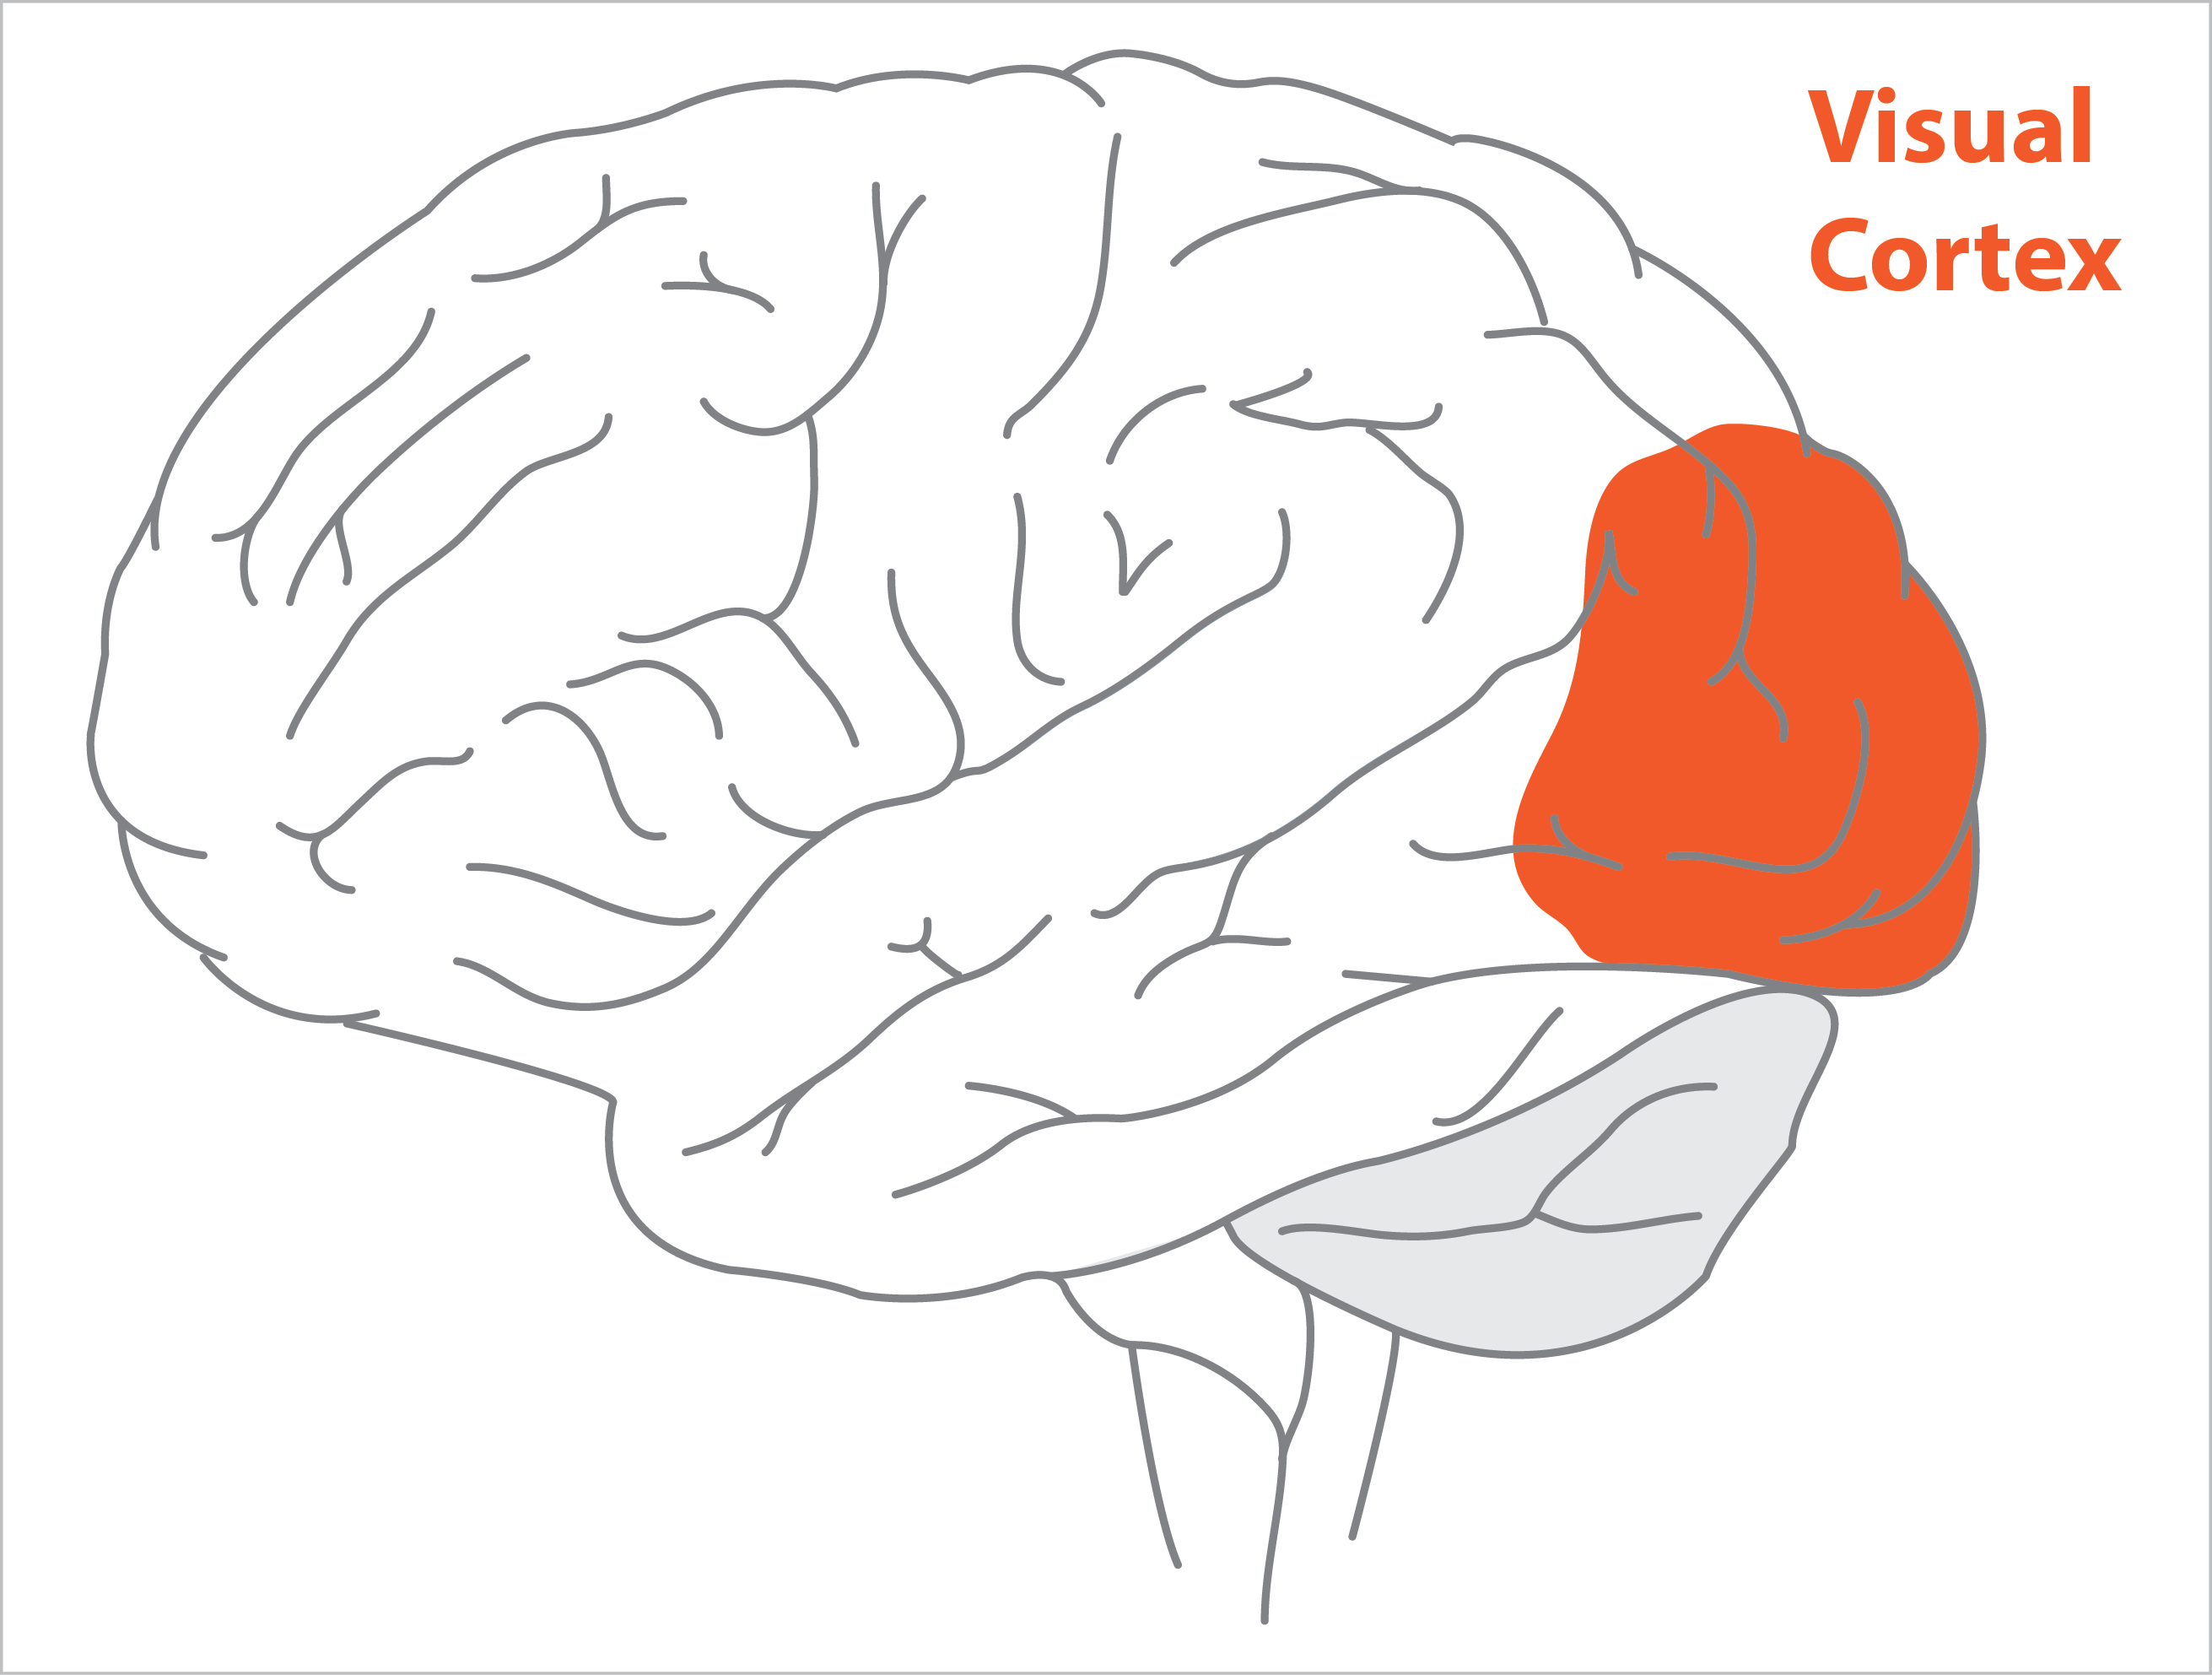
\includegraphics[width=0.8\textwidth]{visualcortex.png} 
                    \caption{Position of the visual cortex. Left is front. Source: \cite{Dr.KenBrodaBahm.14062021}}\label{visual-cortex}
                \end{figure}

                The Sensor will be strapped to the VR headset and thus these two devices will be easy to put on or off.

            \paragraph{Tablet for questions}

                A tablet will be used to collect anonymized demographic data from the participant. This is necessary for the evaluation of the results. See section \ref*{datacollection} for details.

        \section{Remote control interface}
        
            Figure \ref*{gui-remote} shows the interface, which the user will see in the experiment. It resembles the number pad on a conventional TV remote control in structure. The rectangles with the numbers will be the neurotags, where the user has to look at. To measure the activation time, one neurotag will be visually cued - represented by the highlighted \textit{6}. As soon as this neurotag has been activated, a new visual que will be given. The number of occurences in total and of each neurotag will guarantee that the requirements for equation \ref*{itr-basic} will be met.

            \begin{figure}[h]     % h=here, t=top, b=bottom, p=page
                \centering
                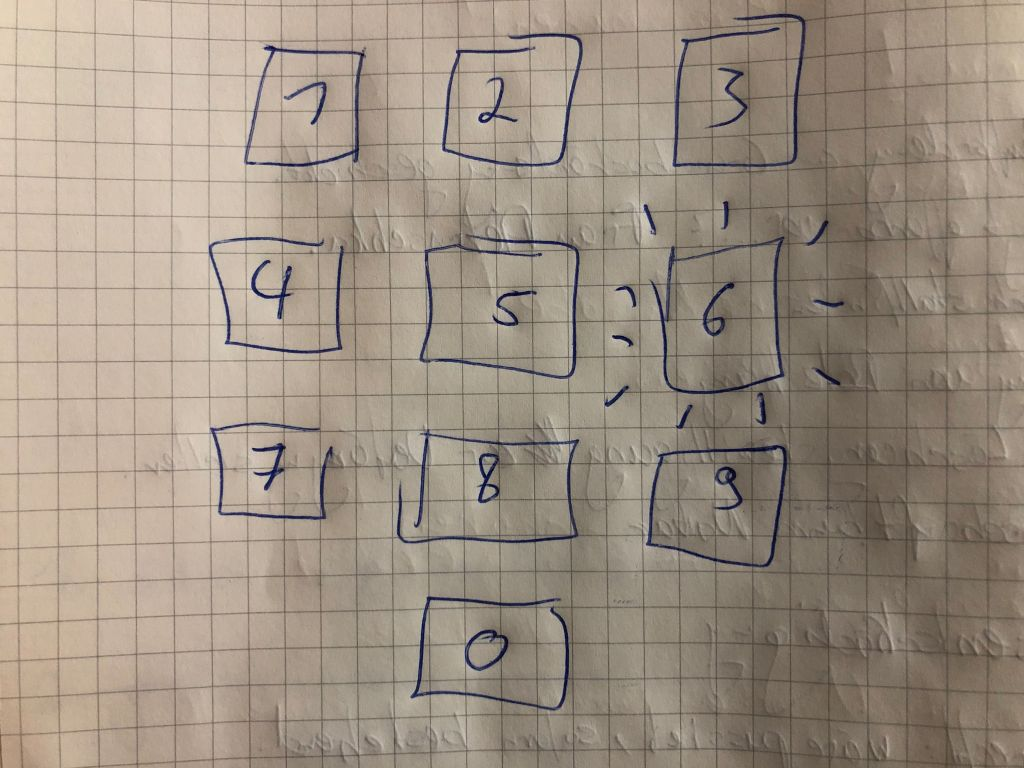
\includegraphics[width=0.8\textwidth]{IMG_8217.jpg} 
                \caption{Layout of the remote control experiment.}\label{gui-remote}
            \end{figure}                    

        \section{What data will be collected}\label{datacollection}

            The data collection will be structured in three blocks: Two questionnaires before and after the experiment which the participant had to answer and data collection during the experiment. The first questionnaire consisted of general questions regarding demographics and medical conditions:

            \begin{itemize}
                \item Demographics: Age and Sex
                \item If the participant wears glasses
                \item If the user felt motion sickness during the experiment
                \item Cognitive impairments
                \item Medication known to affect EEG readings
            \end{itemize}

            The collected data during the experiment was collected on the VR headset (\todo{applicatioin}) and stored in a file, which was available after the finished experiment. This data contained the following readings:

            \begin{itemize}
                \item Speed of each neurotag activation from the point where a cue was given. This is the start of $t1$ until the end of $t2$, where the sensor is confident that a certain neurotag was looked at.
                \item Confidence score of each activated neurotag upon activation until another neurotag is activated.
                \item Quality readings from each single electrode to monitor the tracking quality of the sensor, in order to explain outliers in the collected data.
            \end{itemize}
            
            After the experiment the participant answered the second block of questions, which consisted of questions about the general experience of using the BCI:
            
            \begin{itemize}
                \item If the user felt motion sickness during the experiment (rated 1...5)
                \item comfort of wearing the sensor (rated 1...5)
                \item perceived time to setup the sensor (rated 1...5)
                \item ease of use (rated 1...5) %did it work well?
            \end{itemize}           

        \section{How are the age groups structured}

            To create a meaningful result, the participants have to be divided into age groups.

            \medskip

            \todo{Mail an Prof Lorenz - warte auf Rückmeldung}

        \section{Experimental Protocol}

            The data was collected in a single session lasting around 30mins with each participant. Each session started by the participant having to complete the first questionnaire and the form of consent of their participation. At this stage potential hazards and problems and dispositions as discussed in section \ref{considerations} are identified.
            Afterwards each participant was introduced into the experiment. The working principle of a SSVEP was explained and questions regarding data privacy were discussed. Subsequently the user was shown the GUI of the experiment with a short introduction what the nature of the task was.

            Then the participant was equipped with the VR Goggles and the BCI Sensor (\todo{placed 1m in front of the screen}) and the correct position of the sensor was verified. The first step of the experiment was the calibration of the sensor to the participant. In case of non-optimal readings, the position of the sensor was adjusted accordingly until all electrodes showed at least \textit{very good} contact (figure \ref*{electrode-quality}).

            \begin{figure}[h]     % h=here, t=top, b=bottom, p=page
                \centering
                
\includegraphics[width=0.8\textwidth]{placeholder.jpg} 
                \caption{Quality readings of the sensor}\label{electrode-quality}
            \end{figure}

            Then the experiment was started. The participant was exposed to \todo{50 (?)} different neurotag activations. Each one consisted of a visual que (see figure \ref*{gui-remote}) to which the participant had to focus on. Upon activation of this neurotag, the readings were saved to the logfile the immediately the next cue was given in order to keep the $t1$ timing as short as possible.

            After completion of the experiment, each participant had to fill the second questionnaire, which gathered information such as comford and perceived cognitive load (\todo{find better phrasing maybe?}). 

    \chapter{Survey results}

        \section{Interpretation of the collected data}\label{operationalization}

            Chapter \ref*{doe} provided the necessary framework to decided wheter the hypothesis holds true or not and Chapter \ref*{itr} explains how BCI performance has to interpreted in a given context. This section focusses the contextualization of these metrics in regard to the hypothesis and doe.

            \medskip

            \todo{create coherent argument about ITR and DOE.}

            In regard to figure 2, 3, 4 in \cite{Yuan.2013}: use t1, t2, T and deltaB as argument for performance in experiment.    

                Once the study has been structured and carried out, I can write down the results.

    \chapter{Findings}

        This section also depends on the outcomes in context to the resarch question.

    \chapter{Conclusion}

        \section{Results}

            Summarizing the results and findings of the study briefly.

        \section{Future Work}

            % might be a good suggestion to work on the shortcomings
            % https://www.tandfonline.com/doi/full/10.1080/2326263X.2020.1729652

            Based on the findings and new devices on the horizon, this should give a brief outlook on how to continue this research.

    \chapter{Acknowledgements}

        I want to thank Prof. Dr. Roland Greule and Dipl. Inf. Rüdiger Höfert to examine this study and always set the right impulses to guide the outcome of this thesis. Rüdiger Höfert in particular helped me out with the procurement of necessary equipment to conduct the study. I also want to express my gratitude to the Hamburg University of Applied Sciences to provide the necessary framework to obtain my degree and aid with the procurement of necessary equipment. I also want to express my appreciation for every single participant who took part in my experiments despite certain constraints due to the Covid19 pandemic.
        A special thanks goes to B.Sc. Moritz Bednorz, who helped me sharpen and clarify my knowledge in the field of medical engineering and design of experiment, which gave this thesis a coherent perspective on all domains. 
        I will be eternally grateful to my father Dr. Thomas Neudecker to set the right impulses which made pursue an academic degree. He may rest in piece. 
        My biggest thanks is dedicated to my girlfriend B.A. Alexandra Michels for her emotional support and creative input to some of the figures in this thesis.

    \appendix

        \chapter{Material}

            \section{Surveys, Protocols, etc.}

                Neque porro quisquam est qui dolorem ipsum quia dolor sit amet, consectetur, adipisci velit...

        %--------------------- VERZEICHNISSE ----------------

        \listoffigures % Abbildungsverzeichnis erzeugen
        \listoftables % Tabellenverzeichnis erzeugen

    %--------------------- LITERATURLISTE ---------------
    % Die Einträge sollen alphabetisch sortiert sein.

    \bibliography{references} 
    \bibliographystyle{unsrtnat}

    %--------------------- EIGENSTÄNDIGKEITSERKLÄRUNG ---------------
    \clearpage\thispagestyle{empty}
    \eigen  % im header definiert
    %--------------------------------------- ENDE ------------------------------------

\end{document}